%\section{Introduction}

    This final chapter is intended to describe in some detail the compositional fruits borne of my time spent investigating novel systems of notation. During this project, work always proceeded on two fronts simultaneously: scholarly and creative efforts. As I began developing more robust notions of the syntactic and semantic structure of (open) notations found ``in the wild,'' I increasingly became aware of the subtle but powerful ability of new notations to mediate performance in ways typically closed off to traditional methodologies. As such, I began work on a rather humble framework oriented specifically toward corralling improvising musicians' musical expression with varying degrees of constraint; the ultimate goal being a robust and entirely well-defined scheme with which to play-test structures of fixity-traversal in real time. These creative efforts would culminate in a ``capstone'' concert of original works for a variety of ensembles; each work employing this novel notation scheme in one form or another.
    
    This chapter will serve to document my experiences as a composer-cum-system-developer; beginning with my initial motivations and design concepts, continuing on to details pertaining to the actual structure of the system, and ending with a description and assessment of the capstone works followed by a final reflection evaluating the system's efficacy and future.

\section{Motivations and conception}
    \subsection{Formative experiences with open notation schemes}

    %There were, in essence, two catalysts which eventually led to the work as it exists in its current form; one a ``push'' and the other a ``pull.''
    Over my two years' time in the performance and literature MFA at Mills College (and during my tenure in Oakland thereafter), I was, on many occasions, called to perform by my colleagues and visiting composers. As I was known to be a musician nominally specializing in improvisation, the scores for which I was tapped almost without exception involved some degree of traditionally-notated material as well as some measure of deliberately-incorporated openness. Given the diversity of composerly voices in the program, this openness naturally took many different forms; ranging from flexible, stripped-down traditional notation (à la Berio's \textit{Sequenza I} (1958) to text scores (à la Stockhausen's \textit{Aus den Sieben Tagen} (1968) or any number of Pauline Oliveros' works from the 1970s--1980s) to, of course, ``graphic notation'' which took many and varied forms. The demands placed on these open notations and the goals they were intended to achieve also varied considerably. Composers I worked with sought free-floating Cagean ``aleatory,'' or the shifting densities of Lutosławskian ``stochasticism,'' or the virtuosity of some kind of post-post-bop ``open improvisation;'' each of which seemed to mandate an appropriate graphic trace distinct from our traditional \textit{lingua franca}. Very occasionally, the composer's sound- or process-concept for these open materials would be clear, well-communicated, and artfully and efficiently notated, making for fruitful and relatively painless rehearsals. Far more often, however, these sections (which, to be clear, formed the work's creative core and \textit{raison d'\^{e}tre}) would prove to be intractably difficult to get right, requiring hours of rehearsal, endless composer/performer back-and-forth and, in the worst of times, eleventh-hour rewrites to remove or ``fix'' (literally) the offending material. 
    
    Unfortunately, the extent to which a score was aesthetically interesting or visually expressive seemed inversely correlated with its ability to be successfully ``decoded'' and interpreted. In fact, ``decoded'' is a bit of a misnomer in that new glyphs, where they appeared, would be deployed intuitively; inconsistently---more according to aesthetic principles than musical or conceptual ones. Simply put, in the large majority of cases there was no encoding mechanism in play at all. A series of black dots on a blank field might serve as rather precise rhythmically-proportional notation invoking a precisely-calculated number of pitchless chirps; or, alternately, it might stand in for ametric staccato improvisation within a particular mode. Without a protracted impromptu Q-and-A session with the composer, it was wholly unclear which s/he meant. Problems, naturally, increased in severity as ensemble sizes increased. In the end these experiences became so much the norm that I began to view these notational experiments---especially the ``graphic'' ones---as a lost cause; techniques best replaced by judicious use of explanatory text.\footnote{This is, of course, not to paint every Millsian scored improvisation as irredeemably dire. A number of performances (particularly for small groups whose musicians already enjoyed a degree of familiarity) actually turned out quite well. Where successful rehearsals/performances did occur, however, they tended to be the function of generally pleasant and communicative composers---not said composers' notation design acumen.}

    % \begin{notestuff}
    %     Do I need to actually describe some hypothetical offending graphic scheme...? Visually-impressive but with milquetoast sounds? Barbed wire scores? Or something even more involved-looking but which amounted to chaotic swells? Especially a problem as ensemble size increased...
    %     There was a running joke... <>
    % \end{notestuff}
    
\subsection{Something better}

    % \begin{notestuff}
    %     \begin{itemize}
    %     \item Discovering Roscoe's and Braxton's successful experiments with open notations.
    %     \item Lamenting that I haven't had space to talk about Roscoe
    %     \item Excerpting L-R-G as protoypical successful open notation
    %     \end{itemize}    
    % \end{notestuff}

    Thankfully, while these lackluster firsthand impressions pushed me away from open scoring, I was fortunate enough to be pulled back in, obliquely, by a number of important influences. 

    \paragraph{Roscoe Mitchell}
    Though I had always been particularly drawn to scores as art-objects and had dabbled to a degree with alternative notations, my time at Mills ultimately resulted in access and exposure to many more compositional paradigms than had been available to me prior. In particular, Roscoe Mitchell's composition lessons and group improvisation-sessions proved most valuable in this regard.\footnote{Lamentably, despite my abiding appreciation for Mitchell's works (both as bandleader/composer and with the Art Ensemble of Chicago) I lacked the space in Chapter Three to expand my discussion to these pieces. Mitchell's subtle, highly personal relationship to notation absolutely merits a detailed investigation of its own.} Prof. Mitchell's music had been an important factor in my decision to apply at Mills; since I became aware of his work, I had always been drawn not only to his acute blending of the cerebral and the brute, but also to the constant tension his work seemed to exhibit between clearly improvised material and material which could only have been orchestrated pre-performance. Though I did not know it at the time, Mitchell had developed (among other techniques) a number of simple but sophisticated ways of working with notation that facilitated this blend of fixed/open materials.
    
    Ultimately, my composition lessons granted me rare access to a number of Mitchell's unpublished scores; allowing me to come to grips with some of the ways this was accomplished over the years. Figure~\ref{fig:LRGexcerpt} illustrates an excerpt from one such score: \textit{L-R-G}; a trio for multi-instrumentalists originally written for Mitchell, Wadada Leo Smith, and George Lewis in 1978.  

    \begin{figure}
        \centering
        \fbox{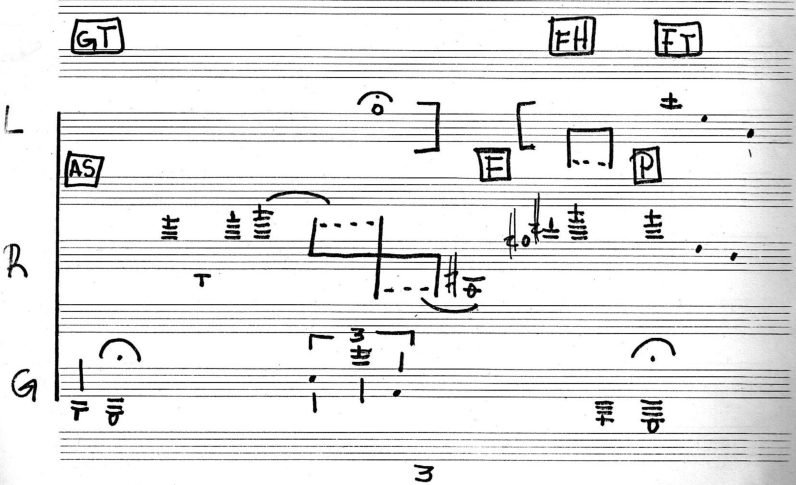
\includegraphics[width=.9\textwidth]{images/chapter4/LRGpg3sys2.png}}
        \captionsetup{width=.5\textwidth}
        \caption{Excerpt from Roscoe Mitchell's \textit{L-R-G} (1978) (pg. 3, sys. 2) demonstrating simple, effective constraint over players' improvised gestures.}
        \label{fig:LRGexcerpt}
    \end{figure}

    \textit{L-R-G} represents a particularly seamless integration of familiar notation with improvisatory inducements of various types. When traditional notation appears, it is, in a sense, distilled to its (pitch + rhythm) essence---much in the same way as one might see in a typical lead sheet. It's clear from the outset that this is a system designed for the creative musician. Where improvisation is called for, it is induced by simple, bracketed portions of the staff---encompassing either the entire staff (as in Smith's first statement in Fig.~\ref{fig:LRGexcerpt}) or only part of it (Mitchell's gesture following the first four notes). Changes of instrument are called for (often in rapid succession) via capital-letter glyphs above the staff (\textit{A}lto \textit{S}ax, \textit{F}lute, \textit{P}ercussion for Mitchell here). Simple rules apply which render the fixed/open gradient transparent; facilitating not only reading but interacting \textit{via} reading. Mitchell demonstrated that meaningful improvisatory interaction could be scored---mediated---via graphic elements while still keeping interpretive ambiguity to a minimum. Indeterminate sound- or process-concepts could be encoded which were nevertheless concretely-defined and well-communicated. \textit{L-R-G}, along with its contemporary ``cousins'' \textit{The Maze} and \textit{S-II Examples} (which all appeared together on Mitchell's 1978 album concatenating the compositions' names) served, in a way, to indict the precious, over-wrought, but ultimately less-than-useful scores I'd experienced prior.\autocite{Mitchell_1978} The crucial difference seemed to be that the score itself served to establish clear rules constraining play; rules which, to be sure, were always fair game to break if need be, but which provided players a default set of parameters clearly communicating the composer's compositional aims.

    \paragraph{Anthony Braxton}
    Likewise, though I was already a card-carrying Anthony Braxton devotee by the time I arrived at Mills, my time with Prof. James Fei (a long-time multi-wind player and Braxton collaborator) exposed me to far more---and more pertinent examples---of Braxton's music, as well as a greater understanding of his sometimes rather opaque working methods. Perhaps paradoxically, the most impactful of these systems was (and remains) Braxton's ``Language Music'' system. Generally, where the Language Musics are cited they appear as a list of twelve glyphs and the gestural families they represent (see Fig.~\ref{fig:language_types} below). 

    \begin{figure}
        \centering
        \fbox{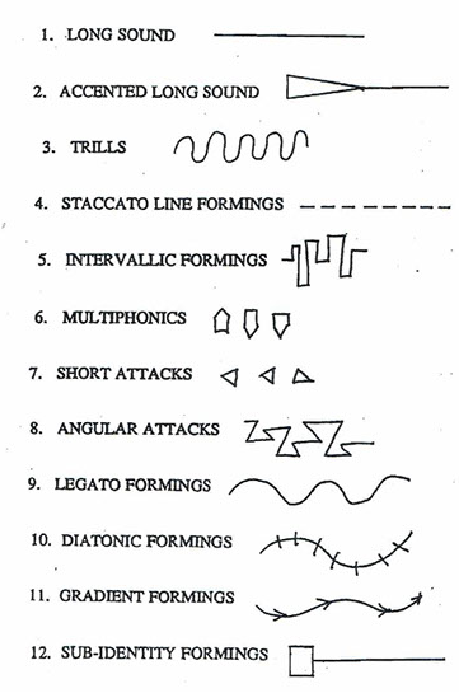
\includegraphics[width=.5\textwidth]{images/chapter4/anthony_braxton_language_types_2.jpg}}
        \captionsetup{width=.45\textwidth}
        \caption[Anthony Braxton's twelve ``language types'' which inform (among other things) his works for unaccompanied alto saxophone.]{Anthony Braxton's twelve ``language types'' which inform (among other things) his works for unaccompanied alto saxophone.\footnotemark}
        \label{fig:language_types}
    \end{figure}
        \footnotetext{\autocite{Lock_1989}}

    \noindent Despite all appearances, though, the twelve language types rarely if ever appear as such \textit{in situ}. Rather than representative glyphs to be used in scores, the language types are better thought of as bite-sized sound- and process-concepts which might be applied in any scored or improvised context. Most famously, they serve as the conceptual framework around which \textit{Composition No. 8A}--\textit{8G} were improvised on Braxton's seminal unaccompanied saxophone album, \textit{For Alto} (1969).\autocite[118--49]{Braxton_1988A} 
    
    The mere fact that something as complex as constrained improvisation could be reduced to simple, two-dimensional glyphs and parametrized in terms of, say, duration and dynamic, again reinforced the notion that improvisers' creative potential could be meaningfully harnessed in the context of a scored work. Given that Braxton demonstrated that well-structured works could be composed using exclusively these gesture-zones (buttressed, of course, by the virtuosic efforts of a stellar improviser), it seemed a comparatively small leap to inscribe these zones on the page in the interest of composer-performer communication.

    Of course, (as demonstrated in the last chapter) not all of Braxton's notation schemata are so simple. Ghost Trance Music, in particular, which I began to study more closely around this time, served as a particularly fascinating example of integrative notation practices. Though the composition scheme would mutate considerably from its inception in the mid 1990s to its current form, Ghost Trance Music bears many consistent features across its instantiations.\autocite{Dicker_2016} Figure~\ref{fig:ghosttranceex} below demonstrates two such features: 
    
    % \begin{figure}
    %     \centering
    %     \fbox{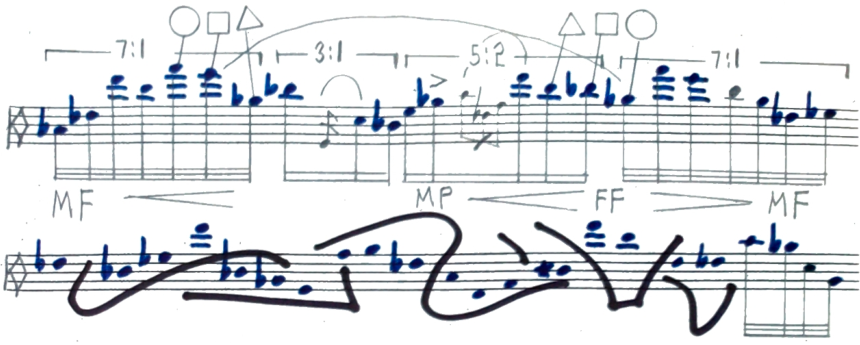
\includegraphics[width=.8\textwidth]{images/chapter4/361pg2sys1.png}}
    %     \fbox{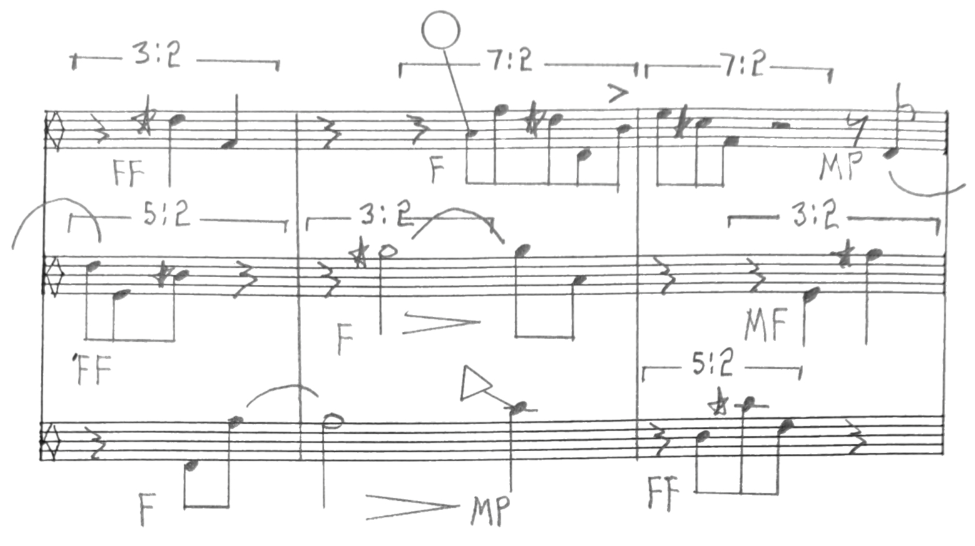
\includegraphics[width=.8\textwidth]{images/chapter4/361secondary.png}}
    %     \captionsetup{width=.5\textwidth}
    %     \caption[Excerpts from fourth-species ``Accelerator Whip'' class Ghost Trance piece \textit{Composition No. 361} (2007) illustrating primary melody (above) and secondary material (below).]{Excerpts from fourth-species ``Accelerator Whip'' class Ghost Trance piece \textit{Composition No. 361} (2007) illustrating primary melody (above) and secondary material (below).\footnotemark}
    %     \label{fig:ghosttrance1}
    % \end{figure}
    %     \footnotetext{Score available thanks to Professor Fei's gracious loan.}

        \begin{figure}
            \centering
            \subfloat[\centering primary melody]
            {\fbox{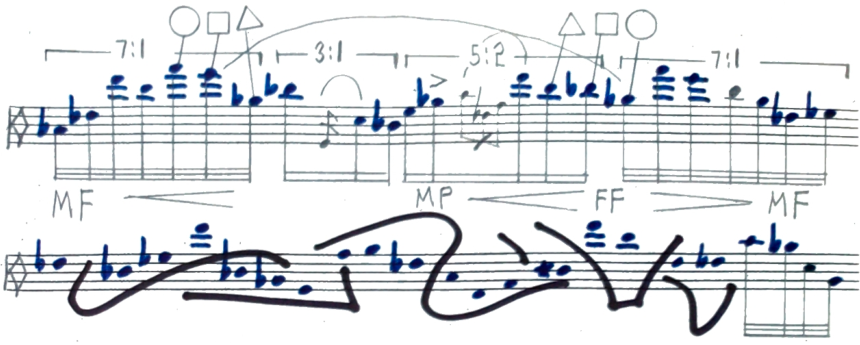
\includegraphics[width=.7\textwidth]{images/chapter4/361pg2sys1.png}}}%
            
            \vspace{5pt}
            
            \subfloat[\centering secondary material]{\fbox{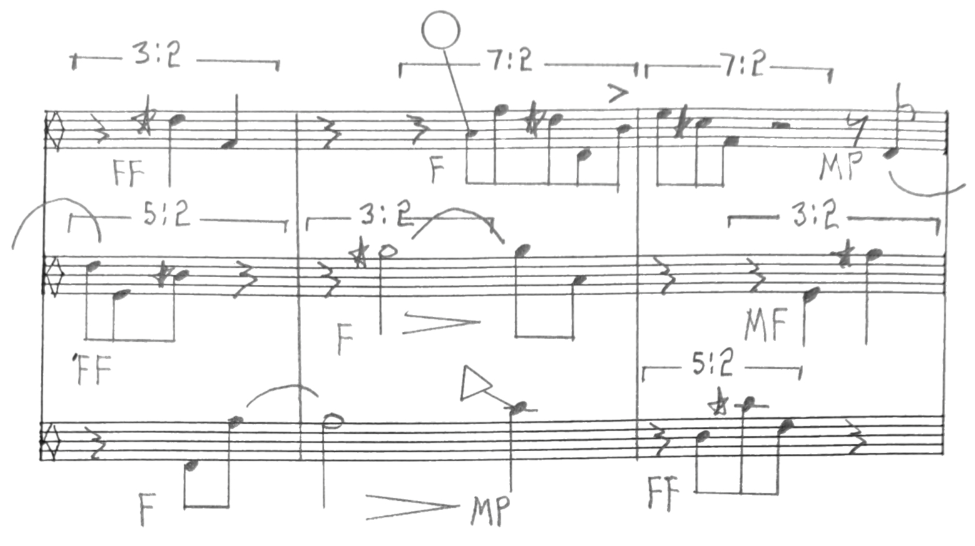
\includegraphics[width=.7\textwidth]{images/chapter4/361secondary.png}}}%
            \captionsetup{width=.5\textwidth}
            \caption[Excerpts from fourth-species ``Accelerator Whip'' class Ghost Trance piece \textit{Composition No. 361} (2007) illustrating primary melody (above) and secondary material (below).]{Excerpts from fourth-species ``Accelerator Whip'' class Ghost Trance piece \textit{Composition No. 361} (2007) illustrating primary melody (above) and secondary material (below).\footnotemark}%
            \label{fig:ghosttranceex}%
        \end{figure}
        \footnotetext{Score available courtesy of a gracious loan by Prof. Fei.---See \shortcite{Dicker_2016} for more details regarding the various Ghost Trance species and classes. }

    Above (a) is a brief excerpt of the ``primary melody''---a long, unbroken melody which wends its way through the entire (often well over an hour long) composition. Where early Ghost Trance works often featured totally isochronous primary melodies sounding as a single, long line of quarter-notes, this late example obscures its primary melody almost entirely with ever-changing tuplets. Below (b) is the ``secondary material''---polyphonic music printed at the end of the score which serves as a reservoir into which performers might jump at particular times to be determined in-performance. Bracketing the minutiae of the system's organization (which deserve a dissertation all their own), I was taken, in particular, by the way Braxton was able to orient a composition around a fixed, unbroken melodic ``flow'' while at the same time building space for several levels of creative decision-making on the part of the performers (decisions which might equally validly be planned out on paper beforehand, hashed out in rehearsal, or arrived at spontaneously in performance).

    \paragraph{Lewis}
        
    Though more limited, I would be remiss not to mention my experience with scholar-composer-performer George Lewis' early work as well. One piece in particular, \textit{Shadowgraph, 5} (for creative orchestra), which formed part of the curriculum in one of our large improvising ensembles, stood out as a particularly economical example of improviser mediation. Figure~\ref{fig:Shadowgraph} gives a single page for the ``saxophone'' group where Lewis combines textual directives, traditional (and modified-traditional) notation in varying degrees of openness, and a single bespoke glyph (the triangle) indicating unconstrained improvisation. Here I was drawn to the work's modularity and flexibility: the piece (like many of the AACM's scored works) is meant to function with an ensemble of any scale and may expand or contract to fit any desired duration. 
    
    Of particular note, though, is the emergent structure of the performer-score interaction. As players navigate the grid, the choice of which sub-module is selected for play is contingent not only on the operant rules-of-play, but also on a continuous stream of sonic and visual data from the rest of the ensemble. The function of the score is to delimit the player's creative choices to adjacent sub-modules while simultaneously demanding a meaningful and relevant contribution to the overall texture within those constraints---a mode of play which strikes me as, in a way, once-abstracted from lead-sheet interpretations. Rather than simply rhythmically or harmonically re-interpreting a lead-sheet symbol to suit the moment's demands, a player (at least in my experience with the work) sits in suspense waiting for the best possible moment to deploy one of the four adjacent sound-zones in their quiver; selecting not the \textit{right note} but the \textit{right mode of play} for a particular scenario. 

    \begin{figure}
        \centering
        \fbox{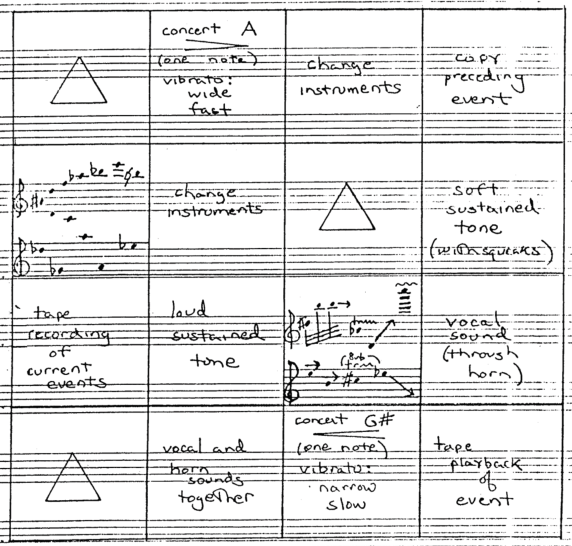
\includegraphics[width=.6\textwidth]{images/chapter4/shadowgraph.png}}
        \captionsetup{width=.5\textwidth}
        \caption[Excerpt (saxophone part) from George Lewis' \textit{Shadowgraph, 5} (1977).]{Excerpt (saxophone part) from George Lewis' \textit{Shadowgraph, 5} (1977).\footnotemark}
        \label{fig:Shadowgraph}
    \end{figure}
        \footnotetext{\autocite{Lewis_1977}}

    \paragraph{New York School}

    Of course my model frameworks extended beyond those of the AACM as well. The New York School, specifically, generally loomed large in the Millsian collective imaginary; both in terms of their theoretical output and their compositional methods. Thus it is no coincidence that in Chapter One I alotted significant space to the unpacking of several new notation methods developed in the 1950s and early 1960s by the likes of John Cage, Morton Feldman, and Earle Brown. Owing, I think, to their relative conceptual simplicity and their ease of adoption by diverse ensembles, New York School compositions repeatedly cropped up in and out of the classroom.

    These artists, steeped though they were in the literate Western art music tradition, treated the score not as a mere afterthought---as a brute archival necessity or a means of mechanically translating S/PC to sound---but as an art object in its own right. However, this focus on the visual never compromised the scores' function \textit{as scores}. Often (excepting, perhaps, the wilder of Cage's scores) golden-era New York School compositions seemed to adopt a Bauhausian functional aesthetic that reduced the notation's inducements and modifiers to their bare essentials: a rectangle for an instrument's functional range; a dot or a line for an inducement to act; its length or breadth a modifier. These were scores which could, in the span of an hour, be picked up and played with little ambiguity as to what, conceptually, the composer was seeking. Figure~\ref{fig:NYS} below is a small, semi-representative sampling of these scores' plain, economical visual traces.
    
    \begin{figure}
        \centering
        \subcaptionbox{Cage---\textit{Aria} \label{fig:cage}}
            {\fbox{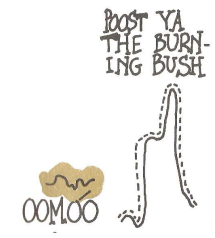
\includegraphics[width=.3\textwidth]{images/chapter4/cage_aria.png}}}
        \subcaptionbox{Wolff---\textit{Edges} \label{fig:wolff}}
            {\fbox{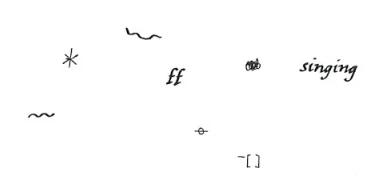
\includegraphics[width=.4\textwidth]{images/chapter4/wolff_edges.png}}}

        \vspace{7pt}
            
        \subcaptionbox{Feldman---\textit{Projection 1} \label{fig:feldman}}
            {\fbox{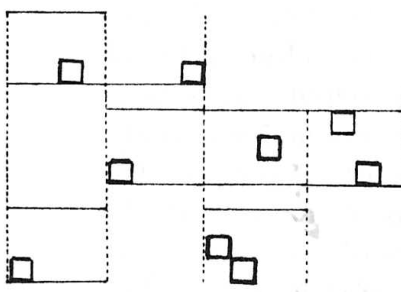
\includegraphics[width=.3\textwidth]{images/chapter4/feldman_projection_1.png}}}
        \subcaptionbox{Brown---\textit{Four Systems} \label{fig:brown}}
            {\fbox{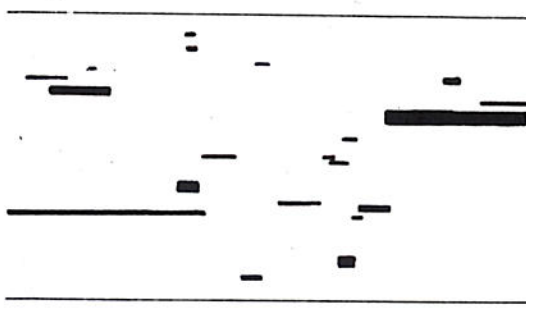
\includegraphics[width=.4\textwidth]{images/chapter4/earle_brown_four_systems.png}}}
        \captionsetup{width=.5\linewidth}
        \caption[(Brief!) excerpts from four semi-representative ``New York School'' compositions demonstrating minimal, comprehensible open notations.]{(Brief!) excerpts from four semi-representative ``New York School'' compositions demonstrating minimal, comprehensible open notations.\footnotemark}
        \label{fig:NYS}
    \end{figure}
    \footnotetext{(a) \autocite{Cage_1958}; (b) \autocite{Wolff_1968}; (c) \autocite{Feldman_1964}; (d) \autocite{Brown_1986}}

    \paragraph{The lead sheet}
    
    Certainly not least among my influences pertaining to this research was my time spent (in various scenes and with varying degrees of dilletantism) as a jazz horn player, guitarist, and drummer. As discussed at some length in earlier chapters, the relationship between jazz performance practice and musical literacy is a complex one. However, it should be safe to claim, at the very least, that the lead sheet model of composition has since the 1940s at latest been the \textit{de facto} standard means of inscribing jazz compositions for easier play, distribution, and archiving (Goodwin's ``TuneDex'' having been introduced in 1942).\footnote{See Ch. 1, ``The Afro-diasporic return to open notation''---\autocite[]{Abel_2016}} As a musician who, for better or worse, has been concerned more with \textit{breadth} of understanding of a given corpus than \textit{depth}, I have typically relied on lead sheets for rehearsal and performance much more than musicians who routinely commit tunes to memory. As such, over the years I slowly became aware of the potent ways the lead sheet's stripped-down glyphs might impact improvised performances. Changing a simple E$\flat^{7}$ glyph into an E$\flat^{7(\flat 9 \sharp 9 \flat 13)}$ has the potential to radically rewrite the field of potential action afforded to a player at a particular point in the composition.

    \begin{figure}
        \centering
        \fbox{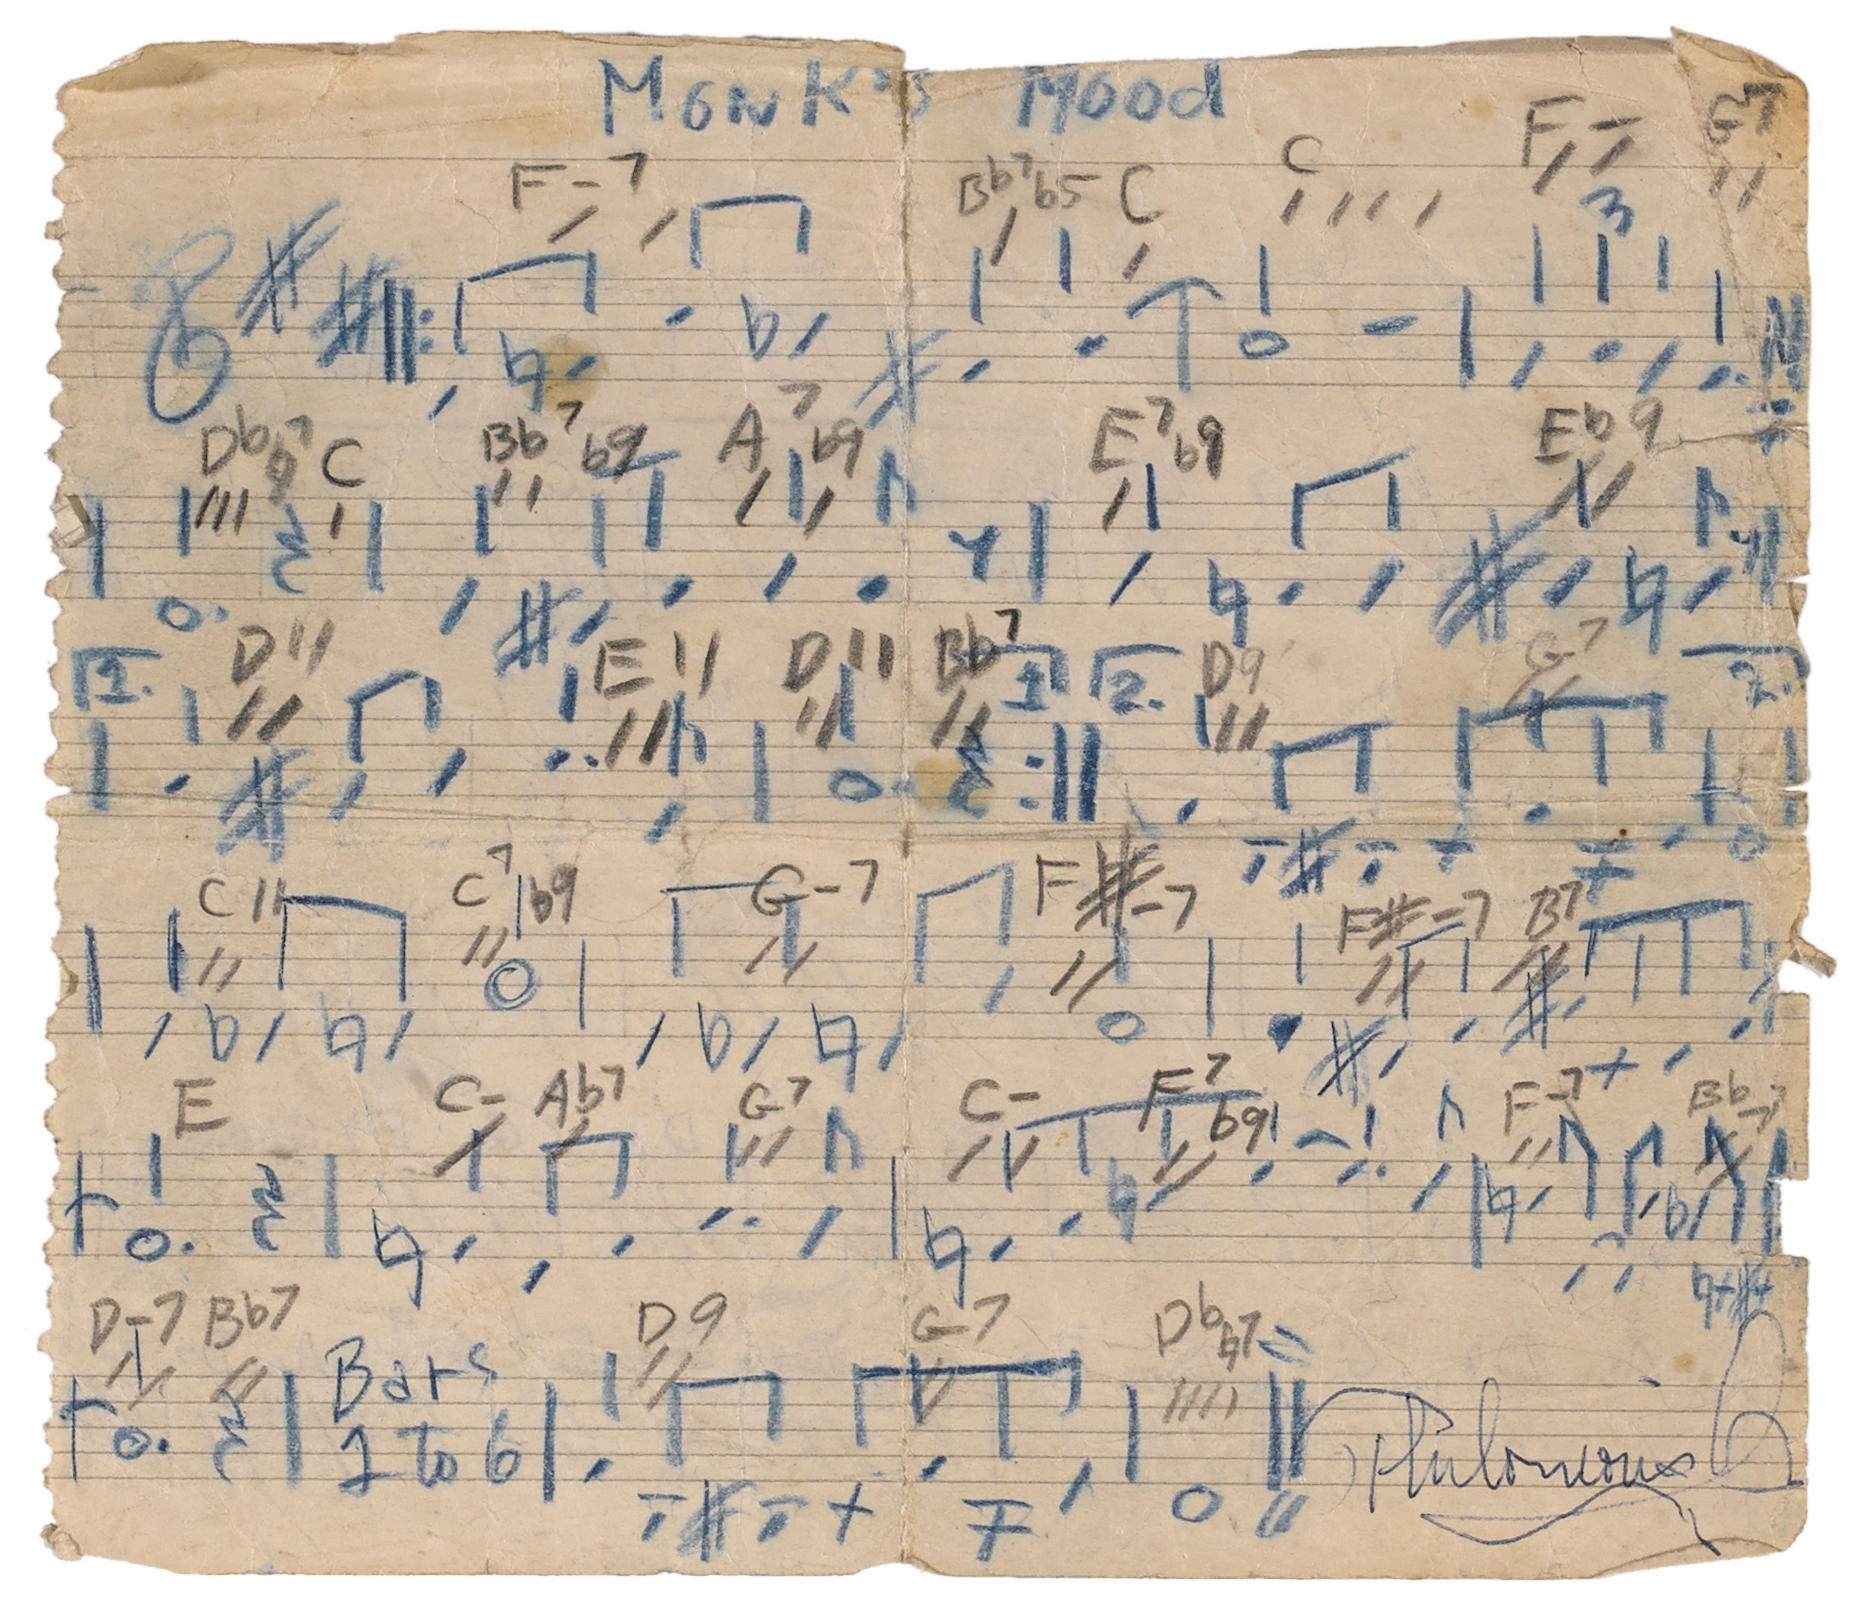
\includegraphics[width=.63\textwidth]{images/chapter4/monk_manuscript_monks_mood.jpg}}
        \captionsetup{width=.5\textwidth}
        \caption[Original manuscript of Thelonious Monk's ``Monk's Mood''. Melody transposed for B$\flat$ instrument.]{Original manuscript of Thelonious Monk's ``Monk's Mood''. Melody transposed for B$\flat$ instrument.\footnotemark}
        \label{fig:monk}
    \end{figure}
        \footnotetext{Sold at Bonhams, 16 June 2015 for \$20,000!---\autocite{Bonhams}}

    (For visual reference, Figure~\ref{fig:monk} provides one such lead sheet: an original manuscript of Thelonious Monk's evergreen ``Monk's Mood'' with the melody evidently transposed for a B$\flat$ instrument.) Lead sheets, after all, represent far and away the most common means of invoking and shaping a collective, creatively-constrained improvisation of any sort. Here as elsewhere, the score does not function as a complete system-unto-itself, instead relying rather heavily on syntactic and semantic standards which musicians must slowly accrue over the course of an entire musical career. However, for those already inducted into the system, the lead sheet (despite typically lacking the usual trappings of traditional scores---dynamics, expressive text, articulations, etc.) bears great power to influence precisely how players approach a tune. This provides an important object-lesson for the would-be notation designer. Namely: the clarity and efficiency with which a notation scheme is able to communicate is often contingent on factors external to the text---specifically the ways in which its users develop a working understanding of its use.

\section{Designing a system}

    Having been exposed to so many laudable methods of writing for improvisers, it became apparent (sometime circa 2020) that the best way to ameliorate the problems I'd faced was (despite all attendant risks) to start work on my own humble notation scheme; ideally aggregating the best attributes of the above (pseudo-)systems while avoiding the pitfalls of haphazardly-constructed one-off ``graphic'' scores. The following section will describe the process by which I designed and implemented such a system. While I'll spare the reader an exhaustive enumeration of each relevant or marginally interesting detail, I will take care to point out particularly thorny or illuminating problems which cropped up along the way.

    This system would be organized around a rather abstract central conceit: that of a sort of ``subtractive'' composition. Traditional notation on the whole might be thought of as a sort of coordinate system which, at its empty ``rest state'' (i.e. a blank score) denotes the musical null set (\O); silence; no play. As symbols are added to the empty canvas of the score, play is induced. A single note represents a single attack with various parameters. Traditional notation is, after all, a system which from its outset (despite its many open forms) was used less for novel creation than for reproduction. If instead we desire the opposite---a system which privileges openness over fixity and production over reproduction---we must begin from the polar opposite standpoint. That is to say: the ``rest state'' of a notation for improvisers should denote the universal set---the set of all possible utterances. For a musician presented with a blank page, all is permitted; the composition denotes no boundaries. The job of our library of symbols, then, must be to pare down this universal set of utterances into a set of potential actions which befits the composer's sound- or process-concept. Here, an action is not built up from silence, but is arrived at through gradual restriction of possible musical moves. The clear analogy here is to two antipodal methods of sculpting. Where the model-maker builds via accretion, slowly adding bits of clay to a form until it eventually resembles some initial work-concept, the stone-carver visualizes a form trapped in the block of alabaster---the set-of-all-forms---freeing it by chipping away unwanted material.

    In truth, not much changes in terms of practical compositional procedure under such a scheme: a composer still selects symbols for interpretation according to some desired sonic or gestural outcome and a performer still interprets them, producing sound. Given, however, that the notation is now organized entirely around varying degrees of variability/indeterminacy, we should expect that such a system should facilitate more complex and interesting forms of open music-making. 

\subsection{Design desiderata}

     Work was quite nebulous to begin with; amounting essentially to a small but growing list of desiderata. The following (presented in loose order of priority) constitute the various ``non-negotiables'' which I saw from the outset as particularly crucial to a functioning notation-for-improvisers.
    
    \begin{enumerate}[label=(\roman*)]
        \item \textit{The system should comprise entirely well-defined glyphs.} Given that the idea to develop a notation scheme in the first place was catalyzed by general dissatisfaction with vaguely- or undefined quasi-symbols, it was critical from the very beginning that each symbol be well-defined and behave identically across instances in a score (or across several scores).\footnote{Again, this is not to somehow denigrate partially or purely-connotative notations which (as I hope Chapter Three has illustrated) can themselves give rise to great art---these are simply the initial boundaries set for the project.}

        \item \textit{The system should adequately balance broad range of potential sonic
        territory with symbolic economy.}   As Pierre Boulez noted in a Coll\`{e}ge de France lecture, 

        \begin{smallquote}
            In the case of known, familiar objects [...] with universal conventions, transcription is a simple matter, but runs the risk of influencing ideas to ensure that they can be included in a familiar mould without special problems. With new objects [...] whose codes are presently uncertain, even non-existent, transcription becomes difficult, imprecise, exaggeratedly complex – complex to the point of uselessness – because one no longer knows how to connect an over-elaborate notation to the object in question. The problem lies in the attention required by the signs defining the object that one wants to communicate – quantitative or qualitative.\autocite[532]{Boulez_Nattiez_2019}
        \end{smallquote}

        \noindent In short, a system of signs is only as good as its ability to be decoded in the context for which it was designed. A system which over-multiplies its symbols in the name of ever-greater representative power runs the risk of requiring too much effort---cognitive, in this case---to decode. On the other hand, a system which is overly-stripped-down in the name of ``readability'' runs the risk of constraining that which it hopes to represent to too great a degree. Thus, any sufficiently mature notation scheme should be able to fluidly negotiate these two factors.

        \item \textit{The system should function equally as a means of transcription as well as performance.}   One of the many strengths of traditional notation is its translational bi-directionality. That is: traditional notation is structured such that a page of well-organized symbols may be realized in sound, but equally that instrumental utterances may be usefully encoded in symbols directly with minimal signal degradation. In other words, a unit of notation's resultant sound is sufficiently tightly-coupled to an instance of a particular symbol that a listener may robustly re-encode a composition from sound alone. This fundamental attribute of the system allows music to be transmitted not only page-to-musician, but musician-to-page. Of course, being that my desired system would deal primarily in variously-constrained improvisation with indeterminate sonic results, it would always demonstrate a lower (read: noisier) signal-to-noise ratio. However, if designed adequately, the system should permit a musician to create a reasonably high-fidelity transcription of an improvisation which otherwise would be quite difficult to represent using traditional notation.\footnote{
            To be clear, the desires for my project differed from those realized in Andrew Killick's ``Global Notation.'' Where his system tailors the notation's encoding methodology to the needs of whatever musical practice is under scrutiny, my transcriptions would always be once-abstracted approximations prioritizing larger-scale clusters of gestures. That said, Global Notation represents a fascinating attempt at solving a centuries-old problem. Because different musical communities build their work-concepts from very different constitutive elements, transcribing a work in Global Notation necessarily involves considering multiple degrees of gestural fixity depending on whether the instrument/practice in question values rhythm over pitch; duration over meter; dynamic over timbre; etc. To that end, for any given instrument it provides a robust means of representing open vs. fixed pitch, open vs. fixed rhythm, and so on. For more information on the motivation behind and use of Global Notation, please see Killick's website.---\autocite{Killick}.
        }
        
        \item \textit{The system should be easily integrated with traditional notation.} Rather than quixotically attempt to replace or subvert traditional notation, I thought it best to incorporate its strengths (not to mention musicians' existing musical literacy) into the new scheme. Thus, the system ought to allow any new glyphs to ``slot in'' alongside more familiar symbols.
        
        \item \textit{The system should be reasonably intuitive to new adopters and sight-readable with minimal effort.} Traditional notation features a number of root-level attributes which persist across nearly all of its instances: regular mapping of time and pitch to $x$- and $y$-axes; left-to-right and top-to-bottom read order; inducement-and-modifier pairings, etc. A new notation scheme ought to preserve these foundational principles so as to facilitate integration with traditional notation and avoid unnecessarily bewildering the reader. 
        
        % \item \textit{The system should be sight-readable with just a little practice.}   Given typical real-world constraints on improvising ensembles (read: limited resources; scant rehearsal time), an over-complicated system requiring constant reference to tables, figures, or other literature would only hamstring performance.
        
        \item \textit{The system should be useful without a strong background in traditional Western musical literacy.} As any sufficiently-experienced musician will tell you, virtuosic talent for improvisation does not always coincide with traditional musical literacy. A successful notation scheme for improvisers, then, should remain accessible even to those ill-versed in Western notation. That is to say: one ought to be able to construct well-formed scores entirely within the system itself.
        
        \item \textit{The system should be easily renderable using pen-and-ink on paper.} Given the utter ubiquity of electronic devices which can engrave or copy arbitrarily complex notation, this bullet point might betray my own aesthetic preferences more than it describes a non-negotiable attribute for a notation scheme. That said, it is unquestionably a boon to be able to quickly jot down an imagined sound-concept or overheard gesture without needing to resort to, say, iPad-specific software or a 3-D rendering engine.
        
    \end{enumerate}

    Armed with these design constraints, I began by narrowing down (a) the parameters I would seek to encode and (b) the visual trace of the notation which would eventually encode them. Initially I imagined the sorts of parameters I would (consciously or unconsciously) consider if I were tasked with ``freely'' improvising in the context of a composition: Would it be rhythmic or arrhythmic? Played with a noisy or pure tone? Involving some sort of imposed tonality or freely atonal? I found it helpful to visualize these parameters as a virtual bank of sliders which might be freely tweaked to suit the composer's desires. For a given gesture, these virtual sliders could either be held constant or varied. The presence of a slider in a particular position meant that its parameter was fixed, i.e. specified by the composer. Its absence would conversely denote an open parameter---one whose state at any given point would be determined by the performer. Thus, the notation's semantic fixity would be continuously variable depending on the specificity of the encoding glyph(s).

    Figure~\ref{fig:sliders} illustrates four hypothetical positions of these imagined sliders which each represent a possible gesture. If it was to be considered a success, the notation scheme would need to be able to represent each gesture distinctly (i.e., either with all parameters fixed in a particular position or with certain parameters fixed and others open) and clearly communicate their relative openness or fixity at a glance.
    
    %Whichever form the notation was to take, it should be able to efficiently encode each parameter given here with enough degrees of freedom to illustrate their change over time (or their absence).

        \begin{figure}
        \centering
        \singlespacing
            \begin{tabular}{|r c l|}
                \hline
                irregular & \texttt{-----|-----------} & isochronous  \\
                noise & \texttt{--------|--------} & sinusoidal \\
                percussive & \texttt{--------------|--} & legato \\
                free atonal & \texttt{--|--------------} & scalar \\
                \lilyDynamics{pppp} & \texttt{--|--------------} & $\lilyDynamics{ffff}$ \\
                romantico & \texttt{-----|-----------} & meccanico \\
                high range & \texttt{---------|-------} & low range \\
                \hline
            \end{tabular}
        
            \vspace{7pt}
        
            \begin{tabular}{|r c l|}
                \hline
                irregular & \texttt{--------------|--} & isochronous  \\
                noise & \texttt{--|--------------} & sinusoidal \\
                percussive & \texttt{--|--------------} & legato \\
                \lilyDynamics{pppp} & \texttt{-----------|-----} & $\lilyDynamics{ffff}$ \\
                high range & \texttt{--------------|--} & low range \\
                \hline
            \end{tabular}
        
            \vspace{7pt}
        
            \begin{tabular}{|r c l|}
                \hline
                irregular & \texttt{--------------|--} & isochronous  \\
                percussive & \texttt{--|--------------} & legato \\
                high range & \texttt{--|--------------} & low range \\
                \hline
            \end{tabular}
        
            \vspace{7pt}
        
            \begin{tabular}{|r c l|}
                \hline
                free atonal & \texttt{--------------|--} & scalar \\
                romantico & \texttt{--|--------------} & meccanico \\
                \hline
            \end{tabular}
        
        \captionsetup{width=.5\textwidth}
        \caption{Four hypothetical parametric configurations for gestures ideally renderable in this as-yet-unnamed notation scheme, from most fixed (top) to most open (bottom).}
        \label{fig:sliders}
        \end{figure}

    The second primary consideration was the form of the graphic elements themselves. Given that these would serve as the tools by which gestures would be encoded as well as an interface for composer/performer communication, it was crucial that their design be well-motivated. From the very start I was particularly drawn to elegance and economy of Braxton's twelve ``language types.'' Although that they were never meant to serve as notation as such, I admired their easy readability, their modularity, and their distinctive, stripped-down aesthetic. While the aforementioned twelve are the most frequently cited and reproduced of Braxton's categories of sound, a cursory glance at the introduction to any of the four volumes of his \textit{Composition Notes} yields a treasure-trove of glyphs and the sound classifications they represent. Figure~\ref{fig:soundclassifications} gives a small sampling of these additional sound classifications not present in the initial twelve. Again, one is unlikely to see these glyphs serving as notation proper while poring over the excerpted compositions themselves. For Braxton, they instead primarily serve to reify a particular S/PC in an quickly-referenceable form---acting more as a mental library of techniques to be deployed in composition in other forms. Like the original twelve language types, though, they provide an excellent model for the notation-designer seeking recognizable, easily-reproducible graphic forms with a high degree of representative power.

        \begin{figure}
        \centering
        \fbox{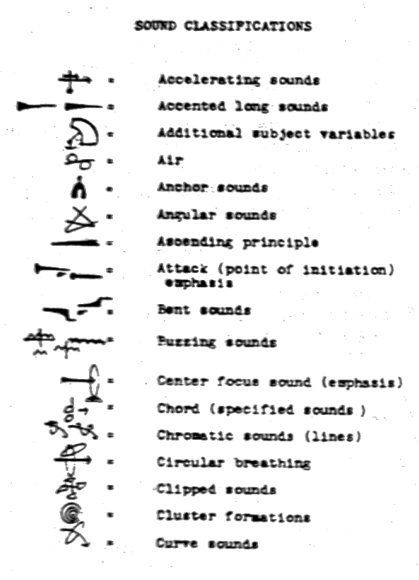
\includegraphics[width=.45\textwidth]{images/chapter4/braxton_supp_1.png}}
        \captionsetup{width=.5\textwidth}
        \caption[Additional ``Sound Classifications'' from Braxton's \textit{Composition Notes}.]{Additional ``Sound Classifications'' from Braxton's \textit{Composition Notes}.\footnotemark}
        \label{fig:soundclassifications}
    \end{figure}
        \footnotetext{\autocite[v-x]{Braxton_1988}.}


    \subsection{Early efforts}

    \subsubsection{Graphic structure}
    My first exercise as fledgling architect, then, was to consider how to represent the twelve language types in my own notation (by now having been given the working moniker ``Otto-Glyphs''---\{O-G\}) such that they might move beyond mere conceptual stand-ins for sounds.\footnote{Please forgive the typographical flourish. Given that ``ogee'' is a term of art referring to serpentine curves (especially in architecture) I couldn't resist the temptation to incorporate curved brackets (comprising four ogees total) in the abbreviated name of the system.} Figure~\ref{fig:braxtonlike2} gives an early sketch of this process. From quite early on, I wanted a way to illustrate both \textit{global parameters} (which would apply across the entire modular gesture) and \textit{local parameters} which might change over its course. As such I opted for an expanded version of Braxton's ``head-and-tail'' format where the ``head'' (the square in Fig.~\ref{fig:braxtonlike2}) initiates the gesture and contains information relating to global parameters and the ``tail'' (the glyphs which follow the head) show its duration and give changing local parameters. Global parameters here might take the form of a key or tonality (B$\flat^{\triangle}$, VII, etc., below) or a technique (growling, sul pont.) and be expressed via text or common symbol in the ``box.'' Local parameters (approximate pitch height, dynamic, attack envelope, silence) would be encoded directly in the ``tail'' itself via a combination of $x$- and $y$- coordinates, stroke weight, and empty space.

        \begin{figure}
            \centering
            \fbox{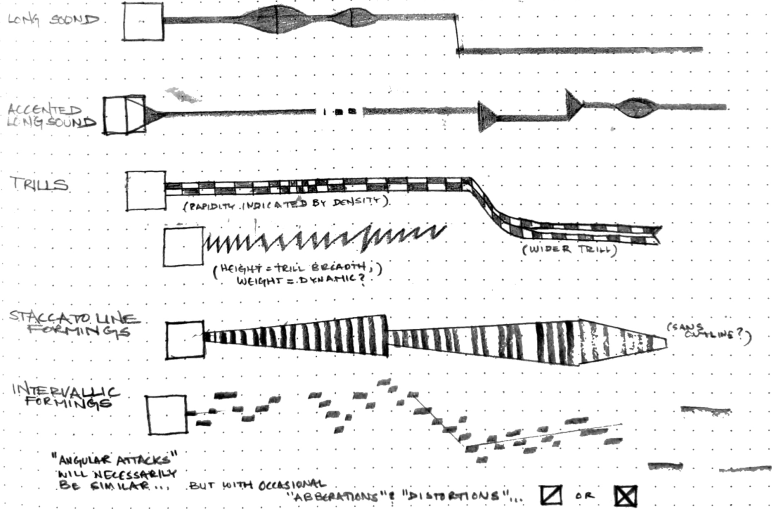
\includegraphics[width=.65\textwidth]{images/chapter4/braxton-like-1.png}}
            \fbox{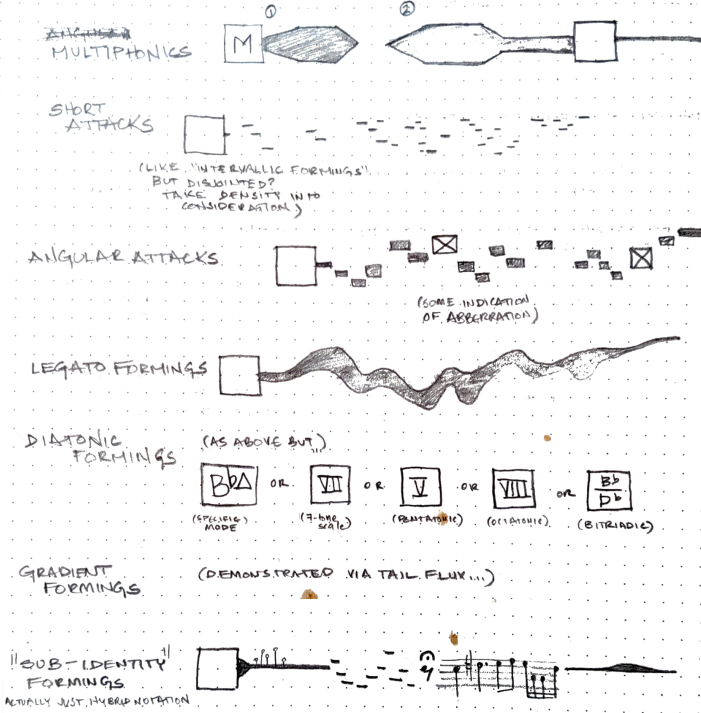
\includegraphics[width=.65\textwidth]{images/chapter4/braxton-like-2.png}}
            \captionsetup{width=.5\textwidth} 
            \caption{An early attempt to render Braxton's twelve ``language types'' into \{O-G\}.}
            \label{fig:braxtonlike2}
        \end{figure}

    \subsubsection{Brackets}
    This exercise alone gave enough shape to \{O-G\} that I could begin experimenting with short scores comprising these types of gestures---leading rather quickly to some key expansions of the system. From the outset, \{O-G\} was conceived as a means of more finely controlling notational semantic fixity---of providing greater or lesser degrees of informational specificity to a performer. What it so far lacked, however, was a way of efficiently communicating rapid, radical changes to this fixity. As we saw in Chapter Three, \textit{Composition No. 76} provided its performers with clear boundaries between gestures which are to be performed (at least loosely) as-written and those which are to form the basis for a more radical form of creative contribution. To achieve a similar clarity, I began to incorporate bracket notation akin to the type used in \textit{L-R-G}. An empty space on the score wrapped by square brackets would denote the aforementioned ``universal set'' of improvisatory gestures---i.e. the direction to ``freely improvise.'' The creative potential for a fixed/open ``on/off'' switch could exceed this simple binary, though. Here I'll quote directly from the user's manual (to be discussed in further detail later in this chapter).

    \begin{smallquote}
            In essence: any time brackets appear, they should be read as: \textbf{play something \textit{in this manner}}. How precisely \textbf{\textit{in this manner}} is interpreted will of course differ greatly between performers. For instance: Where this figure...

            \begin{center}
            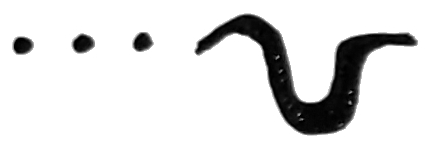
\includegraphics[width=.2\textwidth]{images/chapter4/01-3dotscurve.png}
            \end{center}
            
            \noindent indicates \textit{three short attacks and a brief legato passage} across a particular duration, its bracketed counterpart

            \begin{center}
            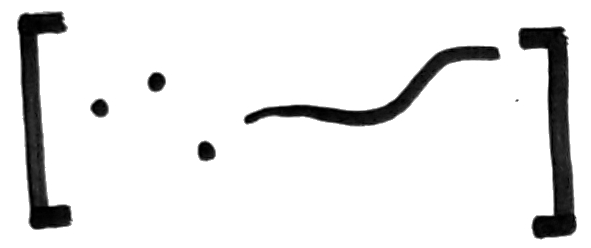
\includegraphics[width=.2\textwidth]{images/chapter4/01-3dotscurvebracket2.png}
            \end{center}
            
            \noindent asks the performer to play using these \textit{sorts of} gestures for the duration indicated by the brackets/arrows. Rather than specify certain sounds in certain orders, the bracketed gesture gives a player a sort of ``sonic territory'' to occupy for a given time. The player ought to feel more ``freedom'' with respect to the execution of the material therein than with the more cut-and-dry plain gestures.\footnote{\textit{Otto-Glyphs}, pg. 19--20, Appendix}
    \end{smallquote}

    To my mind, incorporating this ``rapid-traversal'' mechanism would both (a) provide the player with a visual cue to quickly reconsider the way a certain gesture might fit into the prevailing texture and (b) grant them the creative liberty to reshape the components of that gesture to suit the moment's needs.

    \subsubsection{Relational parameters}
    Another key development which followed initial experiments was the development of signs for cuing and other relational parameters. Braxton's relational codes (as referenced in Chapter Three---\textsc{dom}, \textsc{supp}, \textsc{op}) provided a simple working model for how these might be deployed. It seemed intuitive, though, that these codes might be expanded to allow more a more fine-grained shaping of these inter-musician relationships. By default, any performance practice for which improvisation is a central organizing factor sets up listening-response feedback loops between its performers. Instituting these relational parameters, though, allows this feedback itself to serve as a locus of creativity in a way that is typically inaccessible to composers.

    By far, the best examples of fine-grained relational composition come in the form of conducted improvisations---namely Butch Morris' ``Conduction'' system and Walter Thompson's ``Soundpainting.'' Since I unfortunately lack the space or time to expound in any great depth on the fascinating living notation which forms these systems' foundation, it must suffice for now to briefly touch on the ways they impacted the early development of \{O-G\}.
    
    Admittedly, my firsthand experience with Conduction and Soundpainting was limited to strictly unofficial exercises---sometimes in accordance with the letter of the official manuals and other times in a sort of unholy amalgam of the two systems. Regardless, it is a testament to the efficacy of systems like these that even watered-down or corrupted versions may serve to meaningfully sculpt six, twelve, or thirty improvisers' creative output---even ones with wide variance in level of expertise, reading ability, experience with they system, experience improvising, etc. Despite the fact that the systems differ greatly in terms of central motivating ethos, both systems share general encoding principles: some central organizer (conductor or Soundpainter) incites and modifies gestures elicited from a player or group of players. The conductor then deploys a series of hand- and body-gestures, drawn from a symbolic library of such gestures made known to performers beforehand. Like other forms of notation, these composer-gestures comprise inducements which call for some sounding and modifiers which manipulate the performers' gestural parameters. As improv-centric systems, composer-gestures tend to be oriented toward creative constraint of players' actions---calling for open improvisation which is somehow pared down according to an intended dynamic, tempo, technique, etc. However, both systems feature codes which allow for quite precise inducements, even allowing encoding of precise melodic and rhythmic elements; practically on the order of traditional notation (though, admittedly this represents a comparatively rare use-case).\footnote{\autocite{Morris_2017} and \autocite{Thompson_2006_1}.}

    Naturally, the ``conductive arts'' differ from traditional scoring methods insofar as they allow continuous, live interplay between the players' sound-producing gestures and the conductor's gesture-producing gestures. This allows for compositions comprising pre-planned sequences of signs to be radically altered or abandoned all together if desired. Nevertheless, I came to think of \{O-G\} as a sort of flattened, concretized form of (small-c) conduction. Walter Thompson, in the first of a series of workbooks, lays out the component-level structure of Soundpainting thus:

    \begin{smallquote}
        The 43 gestures in Soundpainting Workbook I fall under 2 general categories: Sculpting gestures and Function signals.

        \vspace{7pt}
        
        \noindent Sculpting gestures indicate \textit{What} type of improvisation and \textit{How} it is to be performed, and Function signals indicate \textit{Who} performs and \textit{When} to begin performing.

        \vspace{7pt}
    
        \noindent \textit{Who}, \textit{What}, \textit{How}, and \textit{When} comprise the Soundpainting syntax. [...] 

        \vspace{7pt}
        
        \noindent The Soundpainting syntax is further broken down into 6 parts:
            \begin{enumerate}
                \item Identifiers (\textit{Who} is performing)
                \item Content (\textit{What} type of improvisation)
                \item Modifiers (\textit{How} to perform the improvisation)
                \item Go gestures (\textit{When} to begin performing)
                \item Modes (a set of parameters affecting specific gestures)
                \item Palettes (sections of notated or rehearsed music, text, choreography, or visual design)\autocite[4]{Thompson_2006_1}
            \end{enumerate}
    \end{smallquote}

    The workbooks go on to provide dozens of directives, denoting a wide range of performer actions from very simple, sound-oriented gestures (``long tone,'' ``hit'') to much more complex ones which actively modulate the degree of performer interactivity in performance. The ``shapeline'' gesture, for instance, requires that performer ``musically perform the physical shape the Soundpainter creates with her/his body---physical graphic notation'' where the ``synchronize'' gesture asks a performer to ``[synchronize] specified material with specific performer(s).\autocite[34--5]{Thompson_2006_1}
    
    Again, bracketing \textit{live} composer interactivity, it was my hope that \{O-G\} could function much in the same way. Systems were already in place which allowed for a parallel ``\textit{Who}, \textit{What}, \textit{How}, \textit{When}'' organizational structure. ``\textit{Who}'' and ``\textit{When}'' are handled in the same way as traditional notation: by position and alignment on the page. ``\textit{What}'' and ``\textit{How}'' are accomplished by conceptually transposing the four-dimensional movements of a conductor into two dimensional black-and-white glyphs. At this point, \{O-G\} only needed more refined ways of establishing and modifying performer-to-performer and performer-to-notation relationships. Figure~\ref{fig:relational1} below illustrates an early attempt to workshop these signs and Figure~\ref{fig:relational2} shows their current form as of time of writing.

        \begin{figure}
            \centering
            \fbox{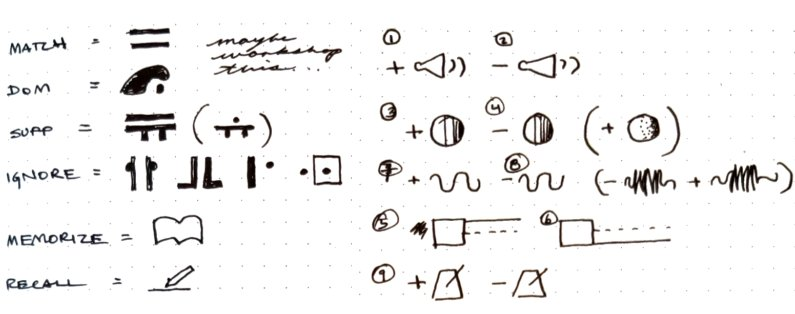
\includegraphics[width=.9\textwidth]{images/chapter4/relationalcombine.jpg}}
            \captionsetup{width=.5\textwidth} 
            \caption{Workshopping relational glyphs.}
            \label{fig:relational1}
        \end{figure}

        \begin{figure}
            \centering
            \fbox{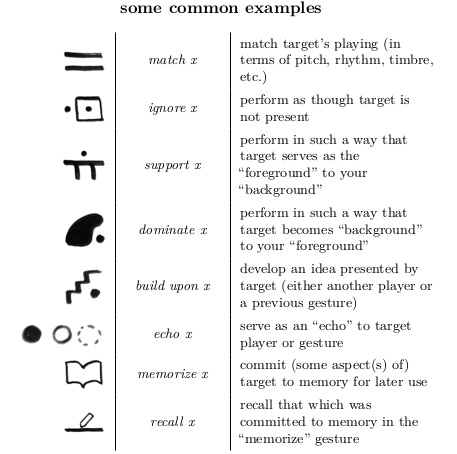
\includegraphics[width=.65\textwidth]{images/chapter4/relationaltable.png}}
            \captionsetup{width=.5\textwidth} 
            \caption{Relational glyphs: current form.}
            \label{fig:relational2}
        \end{figure}

    \noindent Here, ``match,'' ``build upon,'' ``echo,'' ``memorize,'' ``recall'' signs in particular were borrowed from my experience with conduction, while ``dominate'' and ``support'' refer directly to the aforementioned \textit{Composition No. 76}.

    % \begin{notestuff}
    %     Segue to first composition
    % \end{notestuff}

    \subsubsection{\textit{Device for Encouragement of Applause}}

    By this point, with the system having grown to include a basic inducements-and-modifier structure; a means of subtly or radically modulating notational fixity; elements allowing cuing and modification of relational parameters; and now a growing library of basic symbols, the time had come to put the notation scheme into practice. The opportunity to do so arose in 2021 when I was tasked with composing a short (ca. five minute) new work for a mixed ensemble drawn from UC Irvine's ICIT\footnote{Integrated Composition, Improvisation and Technology.} and other music department graduate students.

    The basic theme of the work was the concatenation of two distinct, non-interactive modes of play in a background-and-foreground arrangement. The background---intended to recall a kind of Satiean ``furniture music''---comprised bass clarinet, 'cello, and flute reading from a more-or-less traditional score (Score A) on one extreme end of the performance space.\footnote{In performance: Isaac Otto---bass clarinet, Bella Pepke---'cello, Rebecca Larkin---flute.} Players of Score A self-pace a slowly-pulsed pad of clusters drawn (intuitively, essentially) from an evocative pitch-class set \{0, 2, 3, 4, 6, 7, 9, T, E\} (Messiaen's third mode of limited transposition) which was used as a harmonic reservoir. This pad texture was to loop unobtrusively behind the foreground for the composition's duration. Figure~\ref{fig:encouragementA} gives a one-system excerpt of Score A illustrating a type of proportional notation. Durations of tones and silences are determined by the `cellist's cues.

    \begin{figure}
        \centering
        \fbox{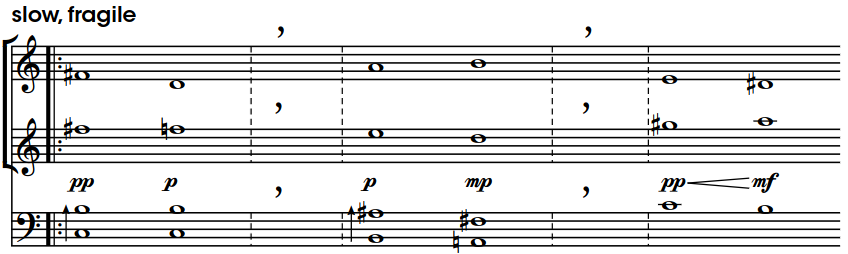
\includegraphics[width=.95\textwidth]{images/chapter4/deviceAsys1.png}}
        \captionsetup{width=.5\textwidth}
        \caption{\textit{Device for Encouragement of Applause}---Score A: System 1.}
        \label{fig:encouragementA}
    \end{figure}
    
    The foreground, on the other hand (Score B) was made up of an improvising duo on trap set and contrabass (located at the opposite end of the space).\footnote{In performance: Steven Lewis---trap set, James Ilgenfritz---contrabass.} Acoustically, I intended that Score B would evoke a chattering, unstable conversation; replete with unexpected, short shouts and frightened murmuring in response. Where Score A would swell and ebb in unison with only the barest inter-musician communication in the form of cuing nods, Score B was to feel more chaotically interactive.
    
    Gestures for the duo were also fully-notated---only now entirely in \{O-G\}. As this was to be the system's maiden voyage, I took care to to limit Score B's vocabulary to only a few distinct types of gestures. This way, I would be able to focus my efforts on assessing and fine-tuning the ways players interacted with the notation rather than on coaching performers on dozens more unfamiliar glyphs. Unlike Score A, which was entirely ensemble-paced, Score B featured no repeats and was paced by stopwatch, reducing the potential cognitive load on relying exclusively on intra-ensemble cues for pacing. Figure~\ref{fig:encouragementB} gives the first page of Score B illustrating this reduced feature-set. Of particular note is the occasionally extreme rate at which the duo here were required to re-assess (consciously or unconsciously) the openness of a given gesture. From the 1'30'' mark to around 2'15'', the bassist must perform two ``in this manner'' gestures (in semi-metronomic time) followed by fixed low tones interrupted by a harmonic---then must execute an open segement with overpressure, a fixed glissando upward, another open segment, and a fixed quiet \textit{col legno battuto} gesture all within the span of around thirty seconds (see Figure~\ref{fig:encouragementB}). While this is not a particularly onerous passage technique-wise, this rapid oscillation between fixed and open modes of play requires a constant renegotiation of one's relationship to the notated material itself (and therefore to the letter and spirit of the composition) as well as to one's bandmates.
    
    \begin{figure}
        \centering
        \fbox{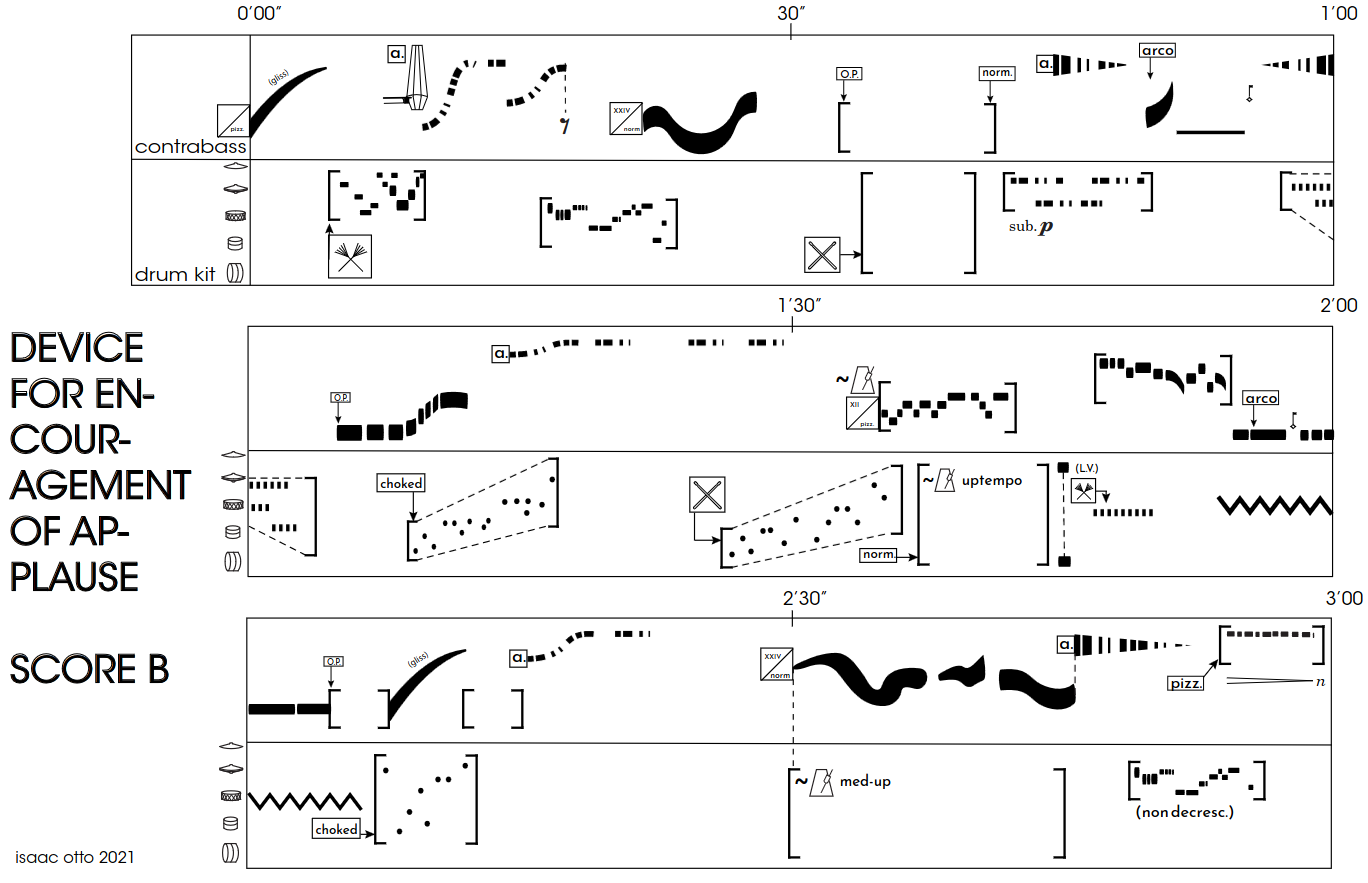
\includegraphics[width=1.3\textwidth,angle=270]{images/chapter4/deviceBpg1.png}}
        \captionsetup{width=.5\textwidth}
        \caption{\textit{Device for Encouragement of Applause}---Score B: Systems 1--3.}
        \label{fig:encouragementB}
    \end{figure}

    \paragraph{Results}
    One key issue which arose during the composition process was that of instrument-specific glyphs. Having primarily performed as a woodwind player for the last decade or so, and having been initially inspired by Anthony Braxton's aforementioned language types (themselves designed around unaccompanied saxophone improvisation), I perhaps inadvertently designed \{O-G\} such that its structure demonstrates a prejudice for pitched, monophonic instruments or at least for gestures which behave monophonically. The fundamental units of notation here are dots (indicating short attacks), lines, and curves (indicating longer attacks undergoing some sort of flux). This did not pose a problem in particular for the bassist here, whose prescribed gestures do not involve any polyphony/homophony and who can happily map pitch to the $y$-axis without any issues. The default mode of play for the percussionist/drummer, on the other hand, is one in which attack durations are determined by the physical structure of the instrument and the initial conditions of the strike. Of course, percussionists have many means of producing swells, drones, and other continuous attacks---but their instrument overall favors polyphony and fixed-duration attacks and does not allow convenient one-to-one pitch/$y$-axis mapping. The solution for the work (eventually titled \textit{Device for Encouragement of Applause}) was to map the individual elements of the drum set to loose spectral regions of the pitch axis---from the kick drum, naturally assigned to the lowest sector, up to the crash cymbal. Note the resultant discrepancy between the average gestural shape for contrabass (fluid, legato, high dynamic contrast) versus that of the trap set (granular, staccato, unspecified dynamic). 
    
    This non-trivial ``translation'' from percussion-gesture space to pitch/time space necessitated further clarification on my part during the rehearsal process. For instance, it was not crystal-clear from the outset precisely how ``pitch'' data within a given instrument-band was to be interpreted; i.e. whether three dots (indicating individual attacks) at different heights on a single ``instrument'' were to be taken to denote different resultant pitches. In this instance (as in the case of other ambiguities which inevitably cropped up), the result was to privilege the demands of the here-and-now in performance. In essence: if the score presents some information which, given a particular performance scenario, doesn't appear to map cogently to any relevant musical parameter, then it should be discarded. If under another circumstance, however, the information presented yields a clear mapping, then it should be executed as faithfully as one deems fit. As a toy example: the player might treat the snare as a temporarily-pitched instrument by applying pressure to the drum-head with the elbow; changing its spectral centroid. In this case, the ambiguous pitch-data are now given contextual meaning and are therefore executable.

    Post-performance, I was heartened by \{O-G\}'s extremely positive performer reception. Though we'd had only precious little time to rehearse, the instructions given with the score in tandem with a few composerly pointers here and there in rehearsal proved sufficient to get at the sound-concept I'd had in mind. Besides the aforementioned percussion-related ambiguity, the notation (perhaps owing to its deliberately simplified construction) was able to both (a) evoke clearly-denoted fixed gestures with predictable sonic results and (b) provide gently ``colored'' space for more open improvisation. Both performers reported that after the initial learning curve, the notation seemed to be able to leave room for creative interplay despite its density and, further, that much to my delight, passing through zones of relative fixity and openness had had a clear impact on their phenomenal experience of the score; that the fixity gradient was actually palpable, even after the signs on the page had begun to be ingrained in memory.

\section{Praxis: composition and concert}

    % \begin{notestuff}
    %     Include full-page figure of the program note front-and-back to begin the section? How do I enforce allowing it to float to wherever it wants despite the overriding rules in the header?
    % \end{notestuff}

    Emboldened by this freshman success I wasted little time preparing for the next two developmental milestones. First, given that even a relatively simple \{O-G\} score (\textit{Device...} Score B) had required a fairly extensive instruction page, I decided to set about creating a formal ``user's manual'' which would serve as the first point of contact between \{O-G\} and its potential interpreters. Formalizing these symbols such that they functioned identically across scores would force me to carefully consider how to articulate not only the ``rules of the game,'' but also my mission statement at large; what, precisely, I hoped to achieve with this humble set of glyphs and most importantly how I hoped to balance composer and performer agency in a system meant to optimize for both.
    
    Second, I made the decision that the ``capstone'' concert marking the culmination of my work in ICIT would exclusively comprise works written (at least in part) in \{O-G\}. The length of the concert would give me the opportunity to demonstrate (via a number of shorter pieces) the system's polyvalence. In particular, I wanted to demonstrate its ability to sculpt a wide variety of sound worlds and to serve the different needs of several diverse performance contexts---whether it be gently shaping otherwise open improvisation or integrating with traditional notation in a particularly fine-grained way. 

    \subsection{Instruction manual}
    \label{sec:instruction-manual}

    %     \begin{notestuff}
    %     Things to discuss here:
    %     \begin{enumerate}
    %         \item Details regarding ``rule breaking'' had to be nailed down ☑
    %         \item Details regarding proportionality/duration ☑
    %         \item Details about curve ``topography''
    %         \item Details about timbral flux
    %         \item Details about lollipops
    %         \item Details about polyphony/homophony (polyphony = several lines = easy, homophony = necessitates new glyphs)
    %         \item The challenge of balancing new glyphs for individual instruments (with individual need) with maintaining a consistent repository of symbols which apply across all instruments. Percussion was one such ``exception''---the voice and especially electronic instruments would require more (but I haven't gotten to them yet)
    %     \end{enumerate}
    % \end{notestuff}

    The central aim of the instruction manual was to digest the feedback (both positive and critical) from performers' experiences with \textit{Device...} and use it in service of a technical document which, while not intended to list each glyph's every conceivable use case, would formally introduce performers to \{O-G\}'s syntax and some of the more common symbols. This necessitated the nailing down of a few more formal features which had theretofore been inconsistently- or poorly-defined---features I will enumerate in part here. For completeness' sake I have provided the full manual in the first appendix for the reader's perusal. 

    Of foremost importance, to my mind, was a robust explanation of the system's take (read: my take) on ``rule-breaking'' as an integral aspect of performance in \{O-G\}. Rule-breaking is, of course, a critical component of any performed music insofar as the performer is always the final filter of the composer's creative intent. A performer maintains exclusive executive control over how music is actually created in that it is their mind, body, and instrument which produce the sound at the end of this causal chain. Certainly, music-making paradigms vary greatly in the degree to which they proscribe or encourage creative rule-breaking. However, I think it fair to say that very rarely is an ``official policy'' ever directly articulated. To rectify this perceived absence, I added the following to the manual's introduction (an excerpt verbose enough, I hope, to not require additional commentary):

    \begin{smallquote}
        Any simple, flexible system of notation such as the one I've sought to realize here could certainly be deployed to suit a wide variety of musical/procedural aims. Indeed it is conceivable that one might, given the right inclination, use this open notation to merely reproduce the traditional composer-over-performer hierarchic paradigm. My goal, however, is precisely the opposite: to build upon the ethos inherent in improvised musics which emphasize co-composition and the \textbf{primacy of the moment}.

        That is to say: in performance, musical situations will inevitably arise which seem to demand a general contribution that runs counter to what is ``prescribed'' in the notation. Perhaps the prescribed dynamic is far too timid for the latent energy of the passage; perhaps a sudden rim shot on the floor tom would propel the music into beautiful new territory---a situation unforeseeable prior to performance. As I conceive of it, the primacy of the moment-in-performance \textbf{demands} that the player heed these calls by making a contribution which deliberately ``disobeys'' that which has been laid out by the composer ahead of time. The notation has already ``done its job,'' so to speak, by sculpting the perceived boundaries of improvisation---it is still incumbent upon \textit{performers} to make the music. I trust the good taste and musical sense of the performer over my prescriptive compositional ability any day. Thus the performer should allow her in-the-moment judgements to supplement and/or override notational prescriptions should the music demand it. Improvised music is decisively a quasi-democratic pursuit---performers should not be shy about \textit{improvising their musico-social roles} as well as the music itself.\footnote{\textit{Otto-Glyphs}, pg. 10--1, Appendix A.} 
    \end{smallquote}

    With this important root-level clarification out of the way, I was able to move on to the task of pinning down some of the more recent additions to the system which I'll quickly sum up here. 

    \paragraph{Proportionality/Duration} I had initially conceived of the system as functioning strictly proportionally---i.e. with duration of a gesture always directly proportional to the extension of the glyph the $x$-axis. However, in the end I opted to grant an additional degree of creative liberty to the performer(s) by allowing that (unless otherwise specified by time stamps, cues, or the presence of traditional time signatures) gestures be durationally-extended as far as the performer desires; so long as the salient features of the gesture itself are proportionally distributed within.\footnote{\textit{Otto-Glyphs}, pg. 15--7, Appendix A.}

    \paragraph{Curve topography} Using curves to indicate melodic contour comes with its own potential issues. Curves in \{O-G\} have consistently been used to represent legato phrases of an approximate shape as opposed to, say, a continuous glissando. As such, a performer might expect that a faithful interpretation of a single (unbracketed) ``S'' curve could involve at most two changes in direction---and likewise that an undulating line would require many, many changes of direction in order to be rendered accurately. It became clear early on that these curves are best thought of as once-abstracted contours that demonstrate larger-scale features of a melodic line and that in realizing them, performers ought to have the liberty to introduce more granular topography than would be otherwise implied. See Figure~\ref{fig:curvebreakdown}.

    \begin{figure}
        \centering
        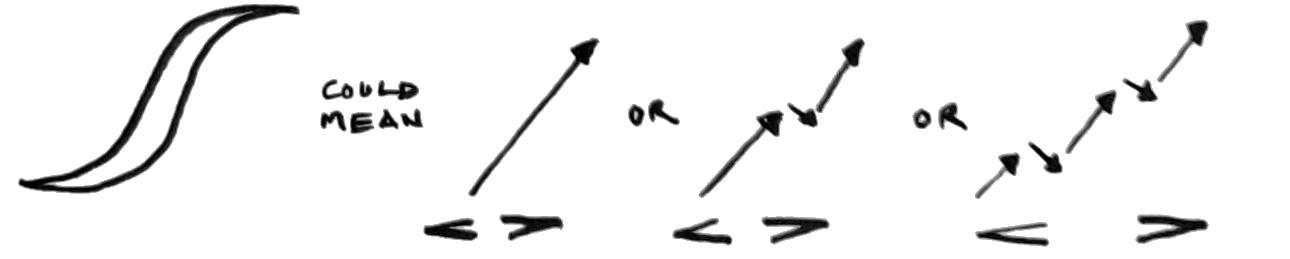
\includegraphics[width=.8\textwidth]{images/chapter4/01-curvebreakdown.png}
        \captionsetup{width=.5\textwidth}
        \caption[An illustration of the several potential interpretations of a simple curve.]{An illustration of the several potential interpretations of a simple curve.\footnotemark}
        \label{fig:curvebreakdown}
    \end{figure}
        \footnotetext{\textit{Otto-Glyphs}, pg. 21--2, Appendix A.}


    \paragraph{``Lollipops''} In testing, the need often arose to proportionally modulate some parameter which was impossible or unwieldy to indicate in the glyph itself. For these situations I began incorporating ``lollypop'' glyphs which would be labeled with the relevant parameter and raised and lowered depending on the parameter's relative state, then connected to indicate continuous (linear) change. This allowed me, for instance, to specify the intensity of a vocal growl for a saxophone gesture or the position of the bow relative to the bridge for a violin gesture (see Figure~\ref{fig:lollypop}).

    \begin{figure}
        \centering
        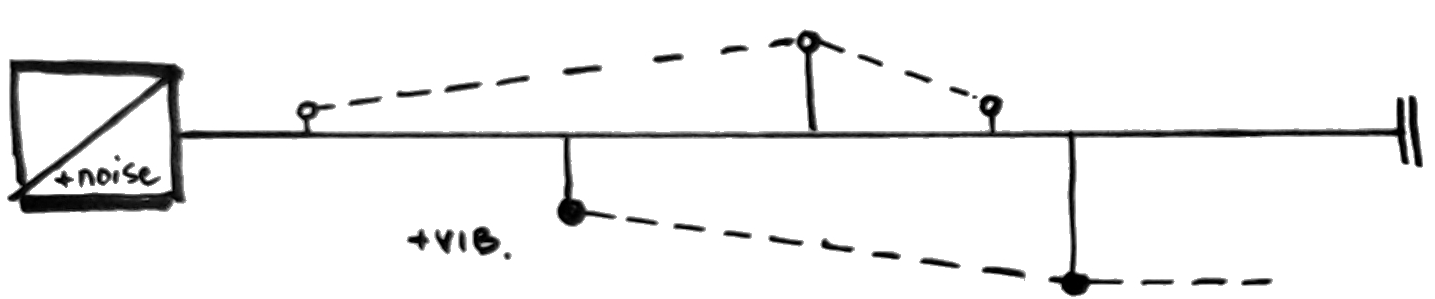
\includegraphics[width=.8\textwidth]{images/chapter4/02-lolly5.png}
        \captionsetup{width=.5\textwidth}
        \caption[An illustration of one potential use of ``lollypop'' glyphs. Two parameters (``noise'' and ``vibrato'') are continuously varied over a stable long tone.]{An illustration of one potential use of ``lollypop'' glyphs. Two parameters (``noise'' and ``vibrato'') are continuously varied over a stable long tone.\footnotemark}
        \label{fig:lollypop}
    \end{figure}
        \footnotetext{\textit{Otto-Glyphs}, pg. 29--30, Appendix A.}

    \paragraph{Instrument-specific glyphs} By the time I finished the manual, I had not yet completed the works for the capstone concert, nor was I certain of the musicians I'd be employing. Nevertheless, I thought it important to include a few instrument- or family- specific glyphs such that I might better tune the compositions to the needs of my future ensembles. (These included, for instance, special textures indicating homophony, specific treatments for double- and triple-stops, multiphonics for winds, harmonics for strings, and mutes for brass.) I mention this not because the chosen glyphs are particularly interesting, but because the notion that family-specific symbols are required at all raises an important question discussed earlier in the desiderata: In designing a system of notation oriented toward (among other things) ease of adoption, how does one responsibly balance \textit{coverage} (i.e. encompassing as broad a range of semantic content as possible) with \textit{economy} (i.e. not employing so many symbols as to over-tax the new player)? In this particular instance, the question is essentially moot; the manual on the whole is only 51 pages long and can be breezed-through in an hour. However, as the system grows to encompass more and more varied performance scenarios, this question will become increasingly relevant. Though I have not yet been tasked with composing a work in \{O-G\} for, say, a modular-synthesist, such an instrument with its many, many manipulable musical parameters could pose a challenge for a system which from its outset was designed around one-line instruments with (comparatively) limited ranges of pitch, dynamic and timbre. See Figure~\ref{fig:homophonic}.

    \begin{figure}
        \centering
        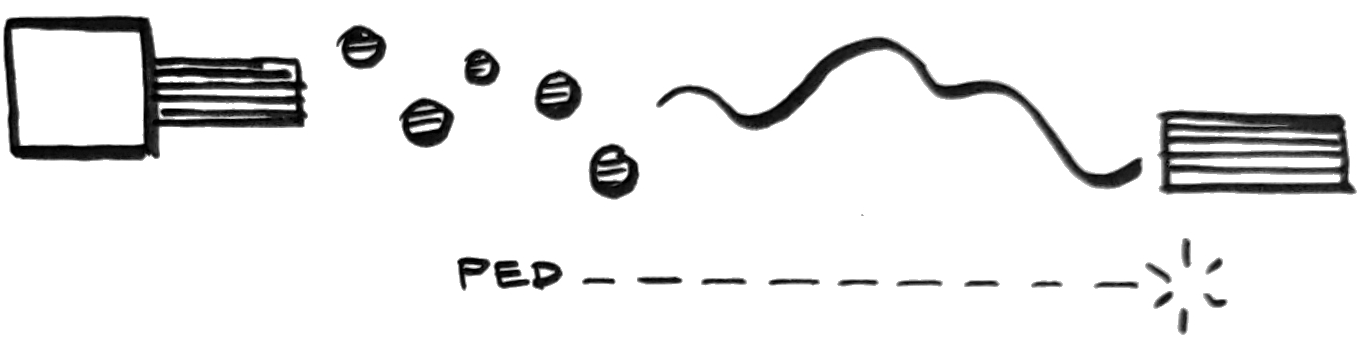
\includegraphics[width=.8\textwidth]{images/chapter4/04-chords5.png}
        \captionsetup{width=.5\textwidth}
        \caption[An illustration of a gesture for keyboard using both homophonic and monophonic textures.]{An illustration of a gesture for keyboard using both homophonic and monophonic textures.\footnotemark}
        \label{fig:homophonic}
    \end{figure}
        \footnotetext{\textit{Otto-Glyphs}, pg. 41--7, Appendix A.}

    % \subsection{Performer response}
    % A number of weeks prior to the final concert, a copy of the manual was printed, hand-bound, and distributed to each performer with the instruction that they were to read and digest it in its entirety prior to the capstone concert's first rehearsal.

    % \begin{notestuff}
    %     Ask Bella about the notes she took in the instruction manual!
    % \end{notestuff}
    
    \subsection{``Capstone'' compositions}
    
    % \begin{notestuff}
    %     One solid paragraph or at most two for each composition! Save any extended commentary for the postmortem.
        
    %     We need a nicely-sized score excerpt for each piece referenced here. \textit{Sostanza} needs a screenshot of the max patch and \textit{Nemat} needs a photo of the instrument layout (or a graphic????).
    % \end{notestuff}

    The compositions selected for the capstone performance consisted of both entirely new works written for the occasion and then-unperformed older works which were adapted in various ways to accommodate \{O-G\}. As discussed above, one important goal of the creative wing of the project was to demonstrate the aesthetic and structural breadth which might be achieved with even a relatively simple notation scheme, assuming it is sufficiently well-defined. As such, I constructed and compiled compositions so as to display this range as much as possible. This section will briefly talk through select compositions; describing what I take to be their most notationally-noteworthy features.

    \subsubsection{\textit{W/M}} 
    
    \textit{W/M} was developed early on as a sort of \{O-G\} \'{e}tude for flexibly-sized ensemble.\footnote{In performance: Isaac Otto---winds, Bella Pepke---'cello, Steven Lewis---trap set, James Ilgenfritz---contrabass. For complete score, please see Appendix C.} Material was presented in the form of a performer-navigable grid of 48 square cells; identical copies of which were given to each performer. Rules of play were constructed such that total duration would remain stable across performances, but that performers would be granted a degree of latitude over the onset and duration of individual cells within the chronological framework. Specifically, performers were to trace a path first from \textit{A-i} to \textit{H-vi} moving only downward or rightward, then upon reaching \textit{H-vi} navigate back to the start moving only upward or leftward. Each cell was to be executed within a thirty-second ``frame'' but might be played at any pace. Thus the cell could occupy the entire frame (leaving no silence) or only a small portion of it (leaving predominantly silence). Performers were meant to remain cognizant of the global sound-world and make creative decisions within this tightly constrained framework in order to bring about the best possible balance of material and silence. Figure~\ref{fig:wmselection} demonstrates twelve modules \textit{in situ}.

        \begin{figure}
            \centering
            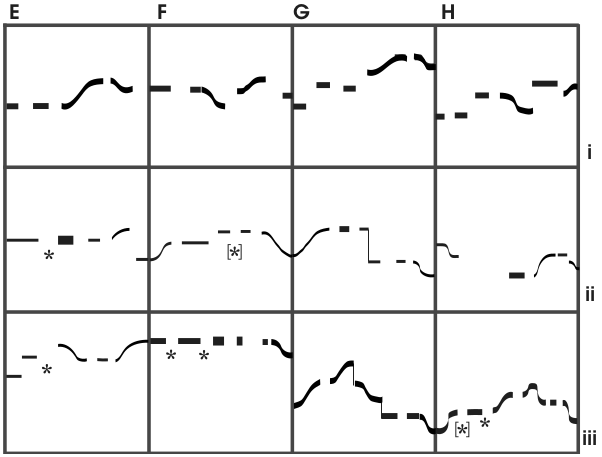
\includegraphics[width=.6\textwidth]{images/chapter4/wmselection.png}
            \captionsetup{width=.5\textwidth}
            \caption{\textit{W/M} excerpt illustrating grid and twelve modules.}
            \label{fig:wmselection}
        \end{figure}

    Given that the work was meant to serve as a primer, the material for each module was drawn from an extremely limited reservoir of techniques: single-tone attacks of various durations and dynamics, short legato phrases, and two types of ``interruptions'' (given by the asterisk and bracketed-asterisk figures). A simple generative scheme was used to construct the work's ``dramatic arc'' (such as it is): Each move away from the origin \textit{A-i} (comprising only a single long tone) adds one degree of complexity to the module which might be a length of silence, a jump in relative pitch, a legato phrase, or an interruption. Thus, as players move toward \textit{H-vi}, they achieve a collective increase in sonic complexity which wanes again as they return to the origin.\footnote{For thoroughness' sake: ``bare'' asterisks represent interruptions to the prevailing texture using any material desired so long as the interruption remains proportional to the cell. As the glyph for the interruption occupies only a small fraction of the space, these should be brief. Bracketed asteriks on the other hand represent ``open'' interruptions which need not be proportional to the durations given in the cell. They might be of any duration so long as they do not violate the thirty-seconds-per-cell rule. Ideally these interruptions (essentially short ``open'' bursts of sound) would introduce enough variety to the material to avoid aural fatigue.} 
    
    To my mind, the limited set of materials and gradual waxing and waning of complexity throughout the piece would both (a) allow players to become more accustomed to ``thinking in'' \{O-G\}; learning to interpret each module as proportionally fixed but durationally open, as well as (b) explore how players use bare-essential materials to construct a cogent sonic landscape according to their personal improvisational aesthetic.

    \subsubsection{\textit{Q-Tet}}

    Where \textit{W/M} presented \{O-G\} in a rather rigorous, ``closed'' form, \textit{Q-Tet} aimed to be precisely the opposite.\footnote{In performance: Isaac Otto---winds, Matthew Nelson---tenor saxophone, James Ilgenfritz---contrabass, João Martins---piano, Atticus Reynolds---trap set. For complete score, please see Appendix D.} The score consisted of four parts---one each for horns, percussion, piano, and contrabass. Each part presented the player with five gestures; four of which were in ``pure'' \{O-G\} and one (at the center of each part) in mixed traditional/\{O-G\} notation. Examples of both of these types are given in Figure~\ref{fig:qtet}. From the outset it was made clear that \textit{Q-Tet} was intended to be first and foremost an open-improvisatory piece---just one that momentarily moved through these five inscribed gestures. As such, beginnings and endings as well as interstitial material were left up to the performers' creative whims. The only requirements vis-à-vis written material were that each (a) each gesture be interpreted at some point during performance, (b) that the gesture marked ``\textsc{first}'' be the first written gesture interpreted and ``\textsc{last}'' be the last, and finally that (c) the central gesture be interpreted as literally/faithfully as possible. 
    
        \begin{figure}
            \centering
            \subcaptionbox{Horns---peripheral gesture.\label{fig:qtethorn}}
                {\fbox{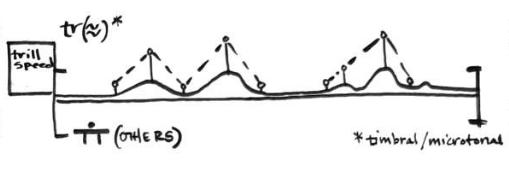
\includegraphics[width=.6\textwidth]{images/chapter4/qtethorn.png}}}

            \vspace{7pt}
            
            \subcaptionbox{Percussion---final gesture.\label{fig:qtetperc}}
                {\fbox{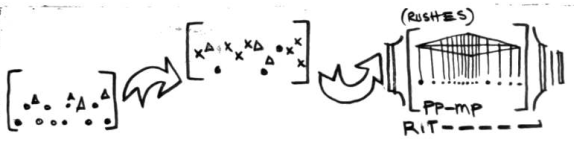
\includegraphics[width=.6\textwidth]{images/chapter4/qtetperclast.png}}}
    
            \vspace{7pt}
                
            \subcaptionbox{Bass---central gesture.\label{fig:qtetbass}}
                {\fbox{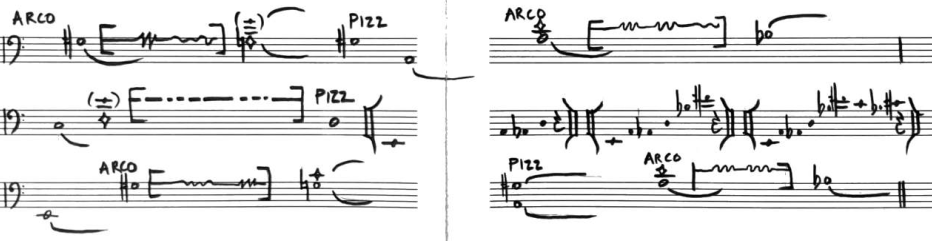
\includegraphics[width=.9\textwidth]{images/chapter4/qtetbasscenter.png}}}
            \caption{Examples of three gestures found in \textit{Q-Tet}.}
            \label{fig:qtet}
        \end{figure}

    Given that nearly all initial, peripheral, and final gestures were presented in brackets, performers were granted a great degree of creative liberty in the way they interpreted or transformed \{O-G\} materials. This was meant to contrast with \textit{W/M}, in which grid modules were (save for interruptions) entirely free of brackets. Given this more relaxed play-environment, I employed more sophisticated notation here: ``transition'' arrows (which prescribe gradual transitions from one sound- or gesture-space to another---shown in sub-figure~\ref{fig:qtetperc}), unspecified parametric ``lollypops'' which require a player to map their own desired parameter to the changing stem-height, and relational modifiers which require the accompanying gesture support other players' expressions (both featured in sub-figure~\ref{fig:qtethorn}). The more-fixed central modules also permitted a degree of experimentation in combining multiple forms of notation, as had always been one of the system's core desiderata.
    
    \subsubsection{\textit{Sostanza come il Sangue}}

    Procedural composition has consistently been a feature (if not a core focus) of my approach; typically used as a means of offloading some creative decision-making to relatively simple algorithms in order that I be able to focus my efforts on some other aspect of composition. These might take the form of sieves which handle the selection of pitches from a central reservoir; the imposition of a dramatic arc via modulating attack density across one movement of a work; or the selection of which simultaneities are to occur between players across an entire piece. As a general rule, I favor conceptually simple algorithms which might, if need be, be worked-out with pen and paper but for which simple programs might be written to expedite this work. \textit{Sostanza come il Sangue} represented my first attempt to rigorously combine a nearly-completely procedural composition with \{O-G\} notation.\footnote{In performance: Isaac Otto---B$\flat$ clarinet, Matthew Nelson---tenor saxophone, Collin Felter---muted tenor trombone, João Martins---piano, Bella Pepke---'cello, James Ilgenfritz---conductor. For complete score, please see Appendix E.}

    Pre-compositional material was developed using a bespoke Max\autocite{MAX} patch in conjunction with \textit{bach}, a third-party package designed to facilitate computer-aided composition.\autocite{Agostini_Ghisi} (See Figure~\ref{fig:sostanzapatch} for patch architecture.) Aesthetically, the overarching goal was to find a sort of twice-abstracted Bach chorale texture which, on the short term, appeared to wander aimlessly but which, over the course of the entire work, eventually found its way to relative stasis. To that end, I sought to generate six non-interactive monophonic lines (tenor saxophone, B$\flat$ clarinet, trombone, left and right hands of the piano, 'cello) which each behaved according to set of simple rules. Each voice was given a central ``destination'' pitch as well as a starting pitch some distance away from it. At any given point, the distance in pitch-space between the current position and the ``destination'' influenced a probability weighting variable. This variable was used to determine whether the pitch in question would remain stationary or move. The further from its destination, the more ``anxious'' and motile it became; as it got closer to home, the less ``desire'' it had to move. In the event that it was selected to move, the pitch had an equal chance to move up or down and by one or two half-steps. Thus, the resultant chords would demonstrate a high degree of parsimony in their voice leading; each voice developed its own independent arc depending on its starting position and destination but the sonic whole was one of smooth chord-to-chord motion. Notes which remained in place were always tied together so as to avoid all voices attacking simultaneously with each step.

    Many, many instances of the program were run with different initial pitches, destinations, and numbers of iterations in order to find a good balance between motility and stasis and to ensure that a few harmonically noteworthy events jumped out over the course of the piece. \textit{bach} was indispensible in that it allowed each run of the software to be visualized in traditional notation and audiated via MIDI within the patch itself. While I ended up tweaking a small handful of pitches toward the end of the piece in order to accentuate the final harmonic ``push,'' the algorithm required pleasantly little interaction on my part and happily generated ten minutes' or so of material with which to experiment. Reviewing the material allowed me to map the emergent harmonies and the ``topography'' of tension-and-release which resulted naturally from six voices in aggregate. 

        \begin{figure}
            \centering
            \fbox{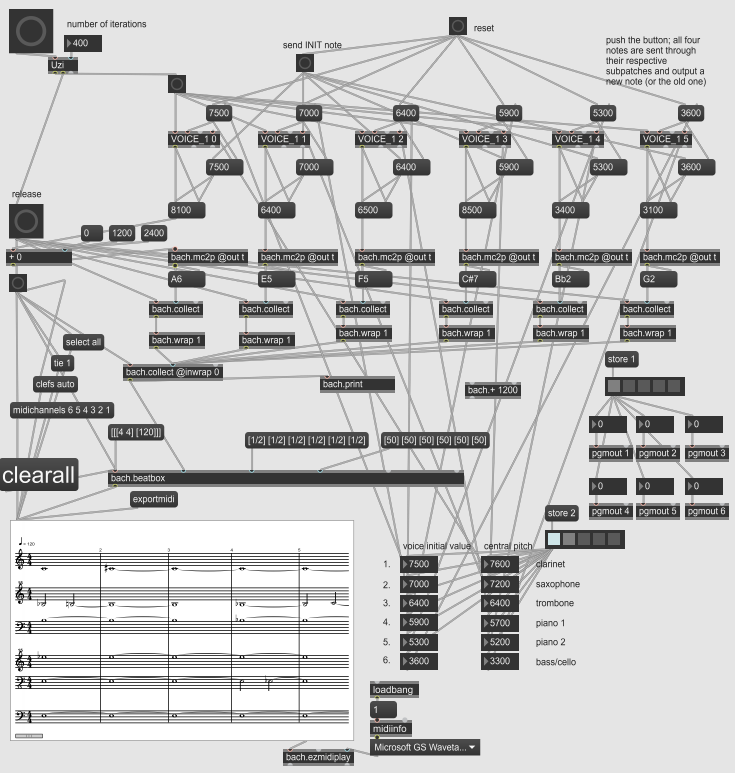
\includegraphics[width=.85\textwidth]{images/chapter4/sostanza_patch.png}}
            \captionsetup{width=.5\textwidth}
            \caption{Max patch used to generate pre-compositional materials for \textit{Sostanza come il Sangue} with the aid of the \textit{bach} package.}
            \label{fig:sostanzapatch}
        \end{figure}

    Integration of improvisatory notation proceeded by excising portions of melodic material from a voice or voices and replacing them with bracketed \{O-G\} gestures. This was done strictly on an intuitive basis; chord members which were of least importance to the emergent harmony (i.e. duplicate pitches, etc.) were most likely to be replaced by new gestures. \{O-G\} elements were kept to relatively simple forms; used, for instance to add a ``micro-improvisatory'' texture (microtonal trills, morse topics, etc.) to pitches already present or providing a series of new pitch classes with which to generate a sub-melody. Glyphs which appeared in dashed boxes were to be performed pitchlessly, e.g. by using only breath or muted strings. Further, players were given the instruction that all improvised elements were meant to be subsumed by the greater harmonic texture---that they should be audible but never dominant. Figure~\ref{fig:sostanzahorns} gives a typical example of the way bracketed glyphs were incorporated with traditional notation.

        \begin{figure}
            \centering
            \fbox{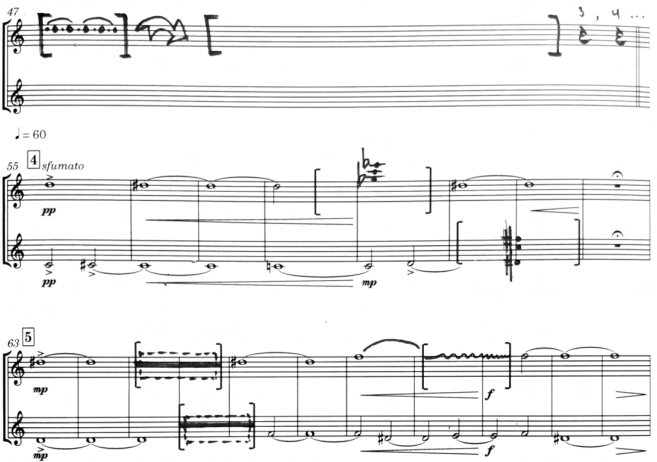
\includegraphics[width=.75\textwidth]{images/chapter4/sostanzahornspg2.png}}
            \captionsetup{width=.5\textwidth}
            \caption{Excerpt from \textit{Sostanza come il Sangue} (top: B$\flat$ clarinet, bottom: tenor sax) horn part illustrating integration of traditional notation with \{O-G\}.}
            \label{fig:sostanzahorns}
        \end{figure}

    \textit{Sostanza...} posed an additional challenge in that it was the first work to bring \{O-G\} into a traditionally-metered context. Performers were challenged to remain aware of their position in the measure while still creatively engaging with the improvisatory directive at hand. This challenge (compounded by limited rehearsal time) was mitigated by including a conductor despite the small ensemble size, as well as by keeping the piece to a comfortable \lilyTimeSignature{4}{4} at $\quarterNote=60$.
    
    \subsubsection{\textit{High Structure Carbon Black}} 

    \textit{High Structure Carbon Black} (\textit{HSCB}) was, if not the first, then certainly the best unaccompanied work for \{O-G\}.\footnote{In performance: Isaac Otto---alto saxophone. For complete score, please see Appendix F.} This score was unique in that it was written to be performed by its author; thus allowing for as sophisticated a vocabulary as I desired. In the end I opted for a diverse but still relatively uncomplicated roster of novel symbols to focus in more closely on just a few techniques (both standard and extended). At its core, \textit{HSCB} took the form of an abstracted lead-sheet with a simple AABA' form, with performance involving several repetitions of this form. The melody itself was composed wholly intuitively, without regard for particular tonic/dominant relations (though in the end, it tended toward a tonic written A$\natural$).

        \begin{figure}
            \centering
            \fbox{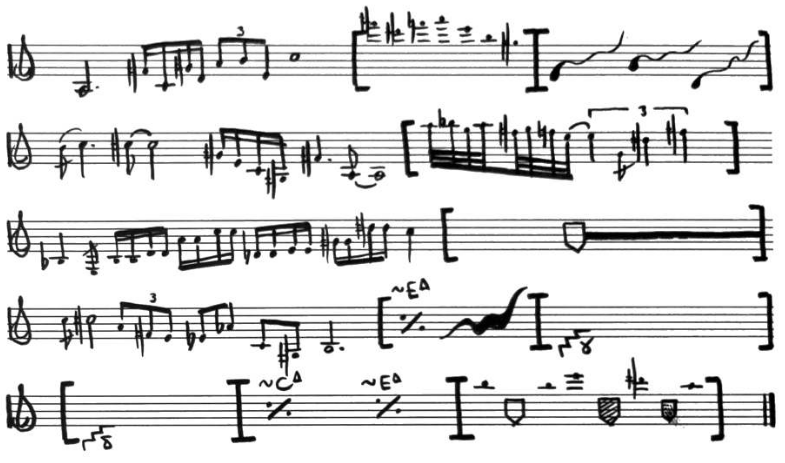
\includegraphics[width=.75\textwidth]{images/chapter4/hscbexcerpt.png}}
            \captionsetup{width=.5\textwidth}
            \caption{Last five systems of \textit{High Structure Carbon Black} (constituting the A' section).}
            \label{fig:hscbexcerpt}
        \end{figure}

    \noindent The single line score contained both traditional notation (sans meter, barlines, and modifiers like articulation or dynamics) and bracketed \{O-G\} glyphs. Borrowing an organization scheme from R\u{a}dulescu, material in brackets was organized into loose gestural regions: $\alpha$ gestures involved stemless pitches with which to improvise, $\gamma$ gestures involved multiphonics, etc. This allowed me to use a class of purely relational gestures such that an empty bracket would be given the relational modifier ``build upon $\alpha$'' or ``build upon $\delta$'' referring back to earlier parts of the score (rather than to other players). Other bracketed gestures included traditional lead sheet symbols (modified with a ``$\sim$'' glyph), legato phrase curves, and combinations of the above. Given that the bracketed gestures remain unconstrained with regard to duration, \textit{HSCB}'s performer is able to (a) modulate the balance between melodic and more open material and (b) sculpt the work's dramatic arc by changing the length of these gestures as they take additional ``choruses.''

    \textit{HSCB} functioned as a loose homage to Braxton's early composition methodology: the bracketed gestures incite exploration of specific sound-zones much in the same way as the ``language types'' aided Braxton in his navigation of the \textit{No. 8} series of compositions on \textit{For Alto}. Limiting the gestural range by only including a few distinct glyphs ensured a general coherence, even in an improvised work that allows considerably more free play than a typical lead-sheet guided performance. 

    \subsubsection{\textit{Nemat-Space}}

    \textit{Nemat-Space} was in some ways the most unconventional (and least systematic) of the entire roster---representing the co-compositional brainchild of performer-composer Niloufar Shiri and myself.\footnote{In performance: Isaac Otto---winds and electronics, Niloufar Shiri---kamancheh and electronics. For full score (such as it is), please see Appendix G.} Over the course of a number of weeks, Shiri and I improvised under loose or entirely absent constraints using a variety of materials (both musical and technological). Over time the composition settled into a multi-layered approach involving several analog recording devices to augment live performance. Freely improvised material and text were recorded onto four-track, stereo, and microcassette. Where the four-track served as a manipulable background layer upon which we would later improvise, stereo and microcassettes became additional tools in a multi-instrument setup which eventually grew to include AACM-esque ``little instruments'' as well (birdcalls, tingsha cymbals, aluminum foil, a length of brass chain, etc).

    Perhaps unsurprisingly given the nature of my work here, finding some way to score these efforts was always a central concern. By the time development of the work-complex was in full swing, I had attempted a number of scoring methods. Figure~\ref{fig:nemat2} illustrates one such attempt.
    
        \begin{figure}
            \centering
            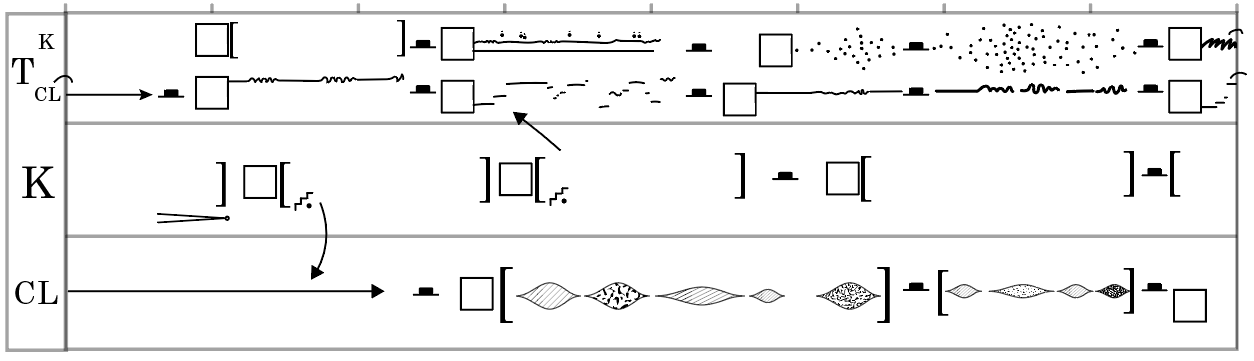
\includegraphics[width=.9\textwidth]{images/chapter4/niloufar_score_long_ex.png}
            \captionsetup{width=.5\textwidth}
            \caption{Excerpt of an \{O-G\} transcription of an early version of \textit{Nemat-Space}}
            \label{fig:nemat2}
        \end{figure}

    \noindent Here, I used \{O-G\} to loosely transcribe events on the four-track tape (first line---marked $T^{K}_{CL}$). Additional layers were then added which only very loosely constrained live players' gestures (primarily using ``build upon'' relational symbols). This sparse notation had the benefit of being able to maintain player orientation over the piece's 15-minute duration and gently corral our playing without delimiting our creative contributions too strictly. In addition, I designed a number of interstitial ``interlude'' scores which would be performed at break-points over the course of the piece. Given that these interludes comprised only one or two gestures each and could easily have been committed to memory, these scores served more as archival documents and/or art-objects than actual performance tools---though they did serve to render this interstitial material far more fixed than the main corpus of the piece itself. Figure~\ref{fig:experimentalinterlude} below gives one such interlude comprising a single long pitchless gesture; giving physical parameters of instrument and microphone placement in addition to the usual prescriptions.
    
        \begin{figure}
            \centering
            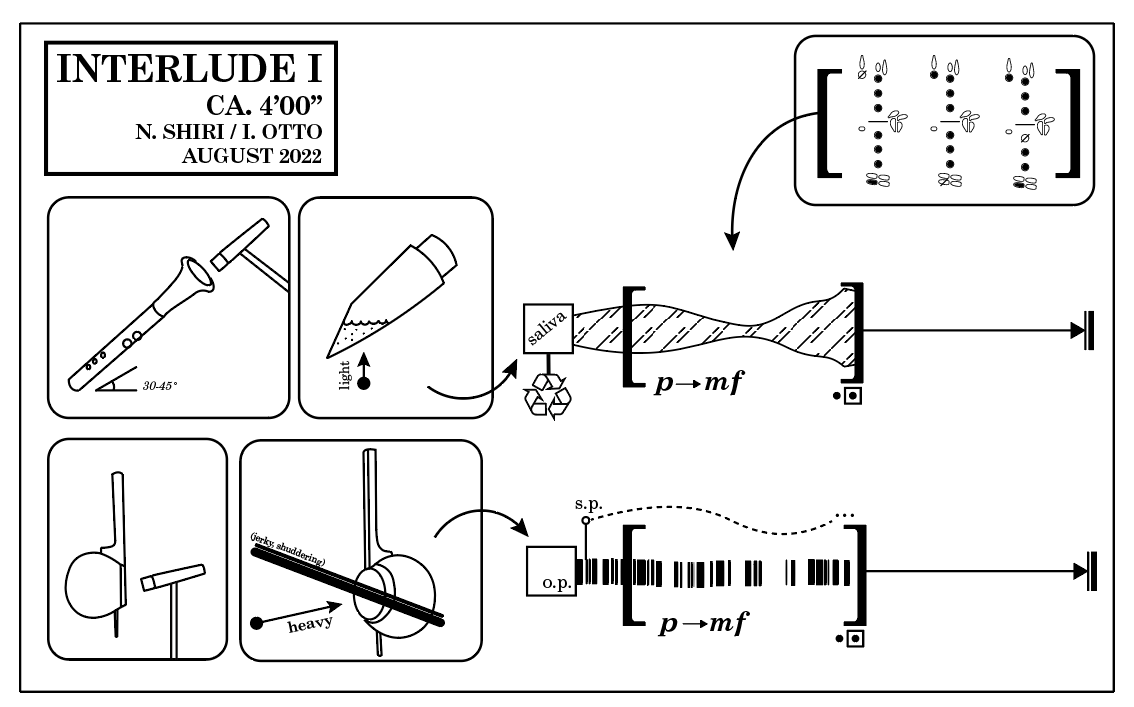
\includegraphics[width=.8\textwidth]{images/chapter4/nemat-interlude.png}
            \captionsetup{width=.5\textwidth}
            \caption{Experimental score for an interlude in an early version of \textit{Nemat-Space}.}
            \label{fig:experimentalinterlude}
        \end{figure}

    After a number of trial runs, we settled on a particular setup and recorded what was to serve as the zygotic form of the final concert-ready piece. In the end, the tools, techniques, and sound-concepts had changed enough that the aforementioned score was shelved (perhaps to one day take on a second life elsewhere) and I started work on an entirely new version based on the physical gestures, sounds, and tape-interactions which emerged during this run. Figure~\ref{fig:nemat2} gives the final one-page score (shown enlarged in Appendix G).
    
        \begin{figure}
            \centering
            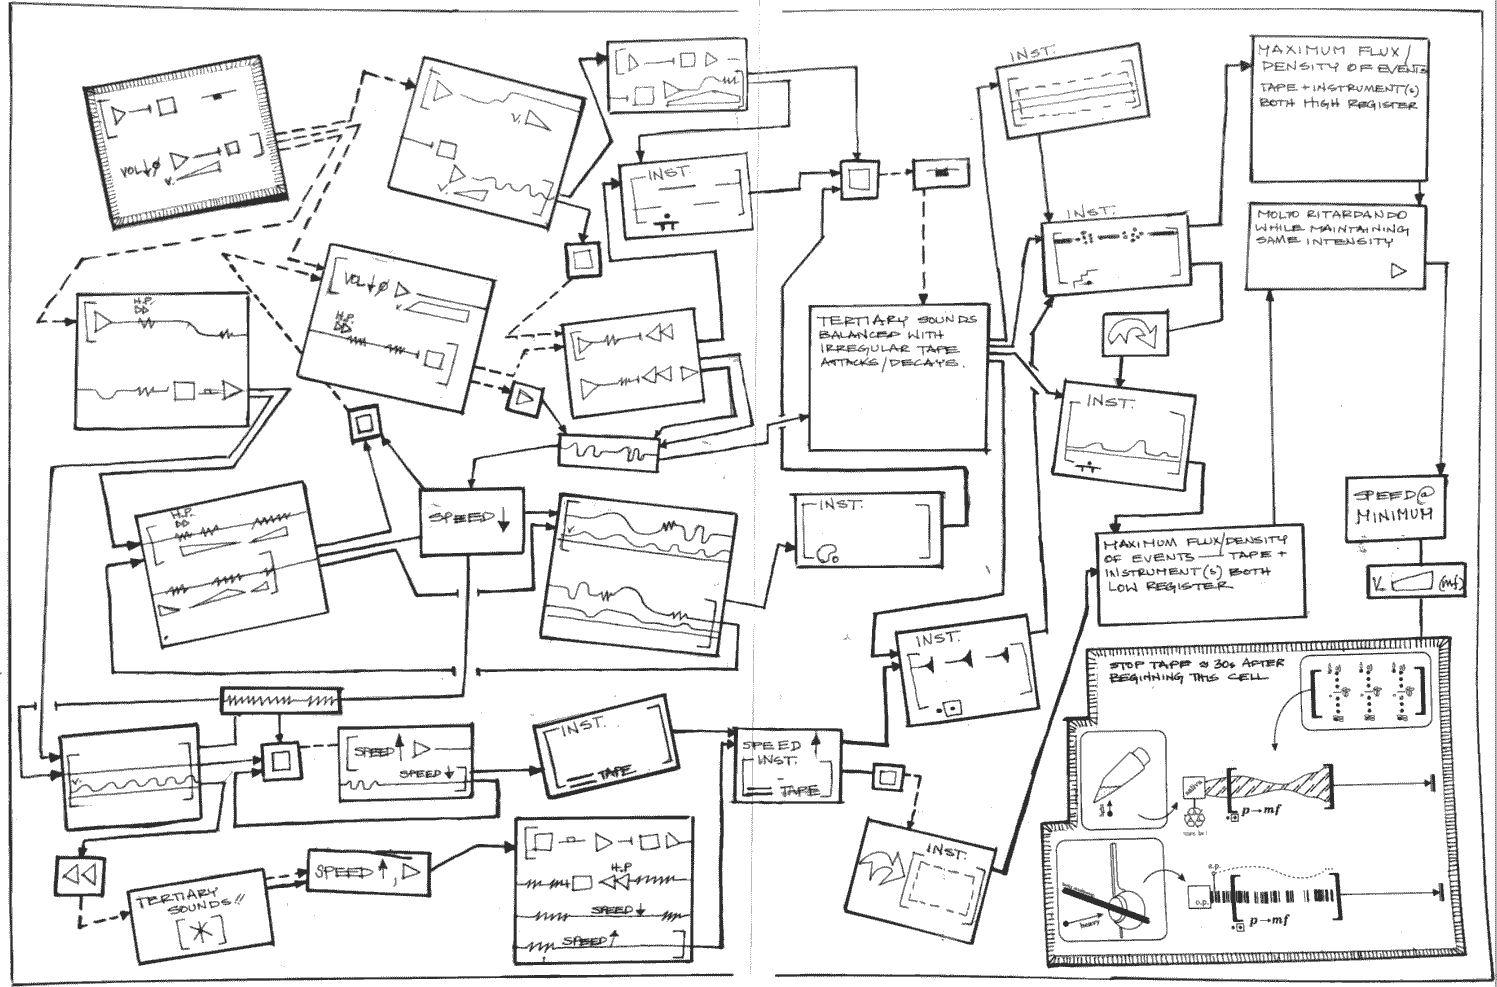
\includegraphics[width=.9\textwidth]{images/chapter4/nemat-space-small-min.png}
            \captionsetup{width=.5\textwidth}
            \caption{Final score for \textit{Nemat-Space}; largely ignored in performance.}
            \label{fig:nematfinal}
        \end{figure}        

    \noindent It is apparent from a glance that this was not a transcription in the same sense as my earlier efforts. Over the course of the co-composition process, we'd arrived at the conclusion that for the purposes of this work, traditional left-to-right linearity was stifling our ability to remain flexible in performance. With this in mind, I approached this score cellularly; with fixed beginning and ending points (note that the earlier interlude was repurposed to serve as the piece's elongated final dramatic gesture). The score's pathing was devised such that some cells provided many branches to potentially traverse, while others featured only one way in or out. The score remained deliberately open-ended with regard to pacing and total duration. Per the central mechanism of the score, performers could only navigate to cells which were linked by arrows (and only in the direction specified). Here I used simple new glyphs to stand in for gestures relating to the tape mechanism: play, stop, rewind, half-press, speed up and down, etc., which were combined with more familiar \{O-G\} glyphs. Material was divided into ``primary'' (gestures performed on one's primary instrument), ``secondary'' (performed on tape devices), and ``tertiary'' (performed on ``little instruments''). Where a gesture or parametric constraint was particularly difficult to express in \{O-G\}, textual directives were employed instead. 
        
    While I have refrained thus far from commenting extensively on the vagaries of performance (which I'll save for the following section), \textit{Nemat-Space} was a special enough case that it demands some further exegesis: In the end, despite having developed what I thought to be a robust conceptual framework and despite having gone through several revisions in order to meticulously balance in-the-moment creativity with composerly intent, our score was almost entirely ignored during the final performance. Given that this was perhaps the most-rehearsed piece on the bill, we had enjoyed a considerable amount of time to internalize precisely the sorts of gestures which best suited our desired \textit{klangwelt} and the rough arc in which they were to be deployed. Thus, while our beginning and ending points remained fixed and while many of the gestures heard in concert corresponded to elements of the score, the document itself was reduced to a library of techniques; really of \textit{reminders} which had no particular authority over the actual activity on stage. All of the meticulously-designed pathwise movement (besides the large-scale arc from ``exclusively tape sounds'' to ``exclusively instrument sounds'') was discarded in favor of an essentially intuitive approach to the piece; sacrificing rigor and reproducibility for a more cogent work which gave itself over entirely to the demands of the here-and-now.
    
    Given that \textit{Nemat-Space} was, to my mind, one of the more successful works on the bill in terms of having attained our desired aesthetic, I consider this an important object-lesson in the broad domain that is writing for improvisers generally. Given that the process began with several sessions of experimentation with techniques and materials, the way in which \textit{Nemat-Space} was co-composed contrasted strongly with the other capstone works which, in a much more traditional sense, left the composer-performer hierarchy intact (albeit modified somewhat). As it turned out, attempting to somehow condense this exploratory ethos to the size of an A3 page and rigorously encode its means of reproduction for an audience was never the right approach. While, undoubtedly, \textit{Nemat-Space} the \textit{score} could under the right circumstances be read literally, methodically; producing an interesting sound-object in its own right, \textit{Nemat-Space} the \textit{work-concept} seemed to resist encapsulation in this way. This is not to say that such work-concepts remain fundamentally incompatible with the notion of scoring generally; only that rendering the ineffable in pen-and-ink might, on occasion, require a new concept of what actually constitutes a score. Clearly, in this instance, the piece was better-served by allowing that the score comprise a non-exhaustive list of available techniques; a series of symbols which serve more of a mnemonic function than an authoritative one. 
    
\section{Postmortem \& Reflection}

    \subsection{Other lessons from performance}

    Of course, this was not the only wisdom waiting to be gleaned from rehearsal and performance. Naturally, there was a strong correlation between the pieces which had had the luxury of multiple thorough rehearsals and the pieces which worked best in practice. I found that principally, when performances were found to be in some way lacking, our problems had more to do with the rendering of traditionally-notated material rather than that of \{O-G\} material---e.g. ensemble blending, intonation, ``tightness,'' etc.---and aren't particularly pertinent to an evaluation of compositional aesthetics or \{O-G\}'s efficacy. Speaking generally, performers were only very rarely unclear as to the parameters constraining improvisation in any particular series of glyphs. However, I did observe an interesting (though not unforseeable) phenomenon whereby players would begin a piece's first rehearsal by rendering gestures (whether bracketed or unbracketed) quite literally despite the creative liberty the symbols were intended to afford. As they grew more comfortable with the material, however, interpretations of bracketed materials began to tend toward greater variability from run to run even without my direct intervention; the lesson being that to a certain degree no amount of specificity of directive can replace practical experience on the bandstand.

    There were only a very small number of occasions where during a player's rendering of an \{O-G\} gesture I observed such a discrepancy between my initial sound-concept and the resultant sound that I felt the need to intervene and clarify precisely what I was looking for. Of course, that these mismatches were not more frequent is as much a testament to the skill of the musicians involved and the bond we'd developed over the (in most cases) several years of performing together as it is to the communicativity of the notation. Nevertheless, I think they merit comment: As I see it, these instances do not reflect some deficiency in the notation scheme or how it is implemented so much as they indicate that reading \{O-G\} can actually be remarkably similar to reading traditional notation. In both cases, during the rehearsal process it is the composer's responsibility to take into account the way performers engage with the written work and amend or clarify as needed such that a balance is achieved between authorial intent and player expectation and ability. 

    Another key observation was that the pieces' notational structure affected a profound impact on performance phenomenology. By and large, the performers I'd selected for the concert were skilled in musical literacy as much if not more as they were in various forms of improvisation. Despite this, where scores were more open-ended with regard to how and when \{O-G\} was to be read, performers seemed to have a much easier time interpreting the notation creatively. Conversely, scenarios where \{O-G\} was constrained by tempo or time stamp, gestures tended to be more dry and literal. As an interpreter myself, I can attest to perceiving two distinct phenomenological modes here. When confronted with floating glyphs which remain temporally untethered, the symbols' gestural content seems to occupy a sort of mental ``memory buffer.'' During play, one has the luxury of waiting (consciously or unconsciously) for the aesthetically most opportune moment to pull them from this ``buffer'' and deploy them when needed. This extends as well to permuting---stretching or squashing---these gestures to best fit the musical moment. This requires a very different sort of creativity than scenarios where a glyph is to be rendered precisely between, say, 2'30" and 2'35". In this latter case, heeding the score's demands seems to take mental precedence over fulfilling some aesthetically-necessary creative impulse; as a result, glyphs are seemingly paradoxically easier to read verbatim (or as close to verbatim as one can achieve under this scheme). I take it that this discrepancy, too, might be exacerbated by limited rehearsal, and that over time even these time-locked gestures could begin to breathe with the same fluidity as more open ones. Nevertheless; given that time is always a luxury for musicians of any sort, these perceptual differences are worth certainly worth bearing in mind for any composer-for-improvisers. 

    \subsection{Reflecting on \{O-G\} as a whole}

    Over the course of the project's design and implementation, I considered five primary criteria with which to evaluate the notation's efficacy. To wit:

    \begin{enumerate}
    \singlespacing
        \item \textit{Ease of acquisition}---i.e. How much trouble did the performer have in learning and adapting to unfamiliar notation? Were there too many moving parts or was the learning curve shallow enough that the players felt that they could meaningfully contribute after sufficient rehearsal?
        \item \textit{Clarity of intent}---i.e. Was it clear pre-rehearsal what the composer was looking for regarding each player's contribution to the music? Or did it only become clear after several grueling hours of hashing-out during rehearsal?
        \item \textit{Engagement with structures of fixity/openness}---i.e. Did the performers find that they could make a clear musical distinction between ``more fixed'' and ``more open'' material and use that to the music's benefit?
        \item \textit{Subjective quality of the final product}---i.e. How engaging or musically stimulating was the performance practice itself? Was the music any good? Or at the very least interesting?
        \item \textit{Novelty}---i.e. Did we achieve something that would, in some way, be closed off to ``pure'' open improvisation or to other methods of scoring?
    \end{enumerate}

    \noindent Upon reflection, \{O-G\} passed \#1., 4., and 5., with distinction. Over the three or so years spent working on the project, as much time (if not more) was spent developing the system's minutiae and ``casting them in stone,'' as it were, in the form of the instruction manual than was spent composing and revising the creative works. Focusing so much of my effort on the clarity and consistency of the encoding scheme virtually ensured that performers would find the acquisition of this new ``language'' easy compared to rehearsing and performing the actual music. Performer feedback here was in essence universally positive; with \{O-G\} being favorably compared to other, one-off systems of notation. The tradeoff here was that this focus on symbolic economy and readability foreclosed certain creative avenues: as deployed, the notation (without some rather severe additions or amendments) could really only be so precise without defeating the spirit of the system. As such, the chosen notation served to ``color'' the compositions in certain ways; simplifying them perhaps, in ways that would not occur to me had I attempted to encode my sound- or process-concepts in traditional notation. 

    In terms of subjective quality of the final product: I consider it the part of the musician's burden to never be fully satisfied with the results of a performance; especially one featuring one's own compositions. There were several instances where I felt that just one or two more run-throughs might have fixed stubborn issues with synchrony or intonation which inevitably pulled attention away from the often stellar creativity on display. However, informal audience polls yielded prevailingly positive responses, especially for pieces where \{O-G\} was featured more front-and-center (i.e. in \textit{W/M}, \textit{Q-Tet}, and the like) and was not in any way compromised by efforts to combine it with structures of traditional notation. The players, too, reported feeling challenged and generally more mentally engaged when confronted with the new scheme than they might feel under other improvisatory modes of play. As desired, the central kernel of the experience for players seemed to be in developing a personal sense of balance between creation and recitation. Most of the music's relative simplicity allowed players the space to cultivate this balance rather than devote precious practice time to the execution of precisely-notated complex phrases. Of course, this, too, came at an obvious cost: several pieces were left on the cutting-room floor owing to their complexity, length or difficulty; compositions which could have served to demonstrate even further creative range. Fortunately, not every goal need be met in a single concert; in the future, more focused creative efforts (say, using exclusively the lead-sheet model of composition as a vehicle for further \{O-G\} development) might pick up where this left off.

    ``Novelty,'' too, I think was an easy win. It is known (at least in the various improv circles of which I've considered myself a member) that as the size of the improvising ensemble increases, so too do the odds that any given open improvisation will inevitably fall prey to a kind of ``curse of the swell.'' This is an (unfortunately? amusingly?) common trope whereby the only noteworthy structural feature of an improvised piece is its slow, large-scale crescendos and decrescendos---by far the easiest sonic features for less experienced improvisers to latch onto and complement. In a certain sense, so long as \{O-G\} was able to circumvent the curse of the swell by facilitating more nuanced and interesting structural features, I would have counted it as a success. An undeniable strength of the scheme is that even barely-constrained improvisation denoted primarily by empty brackets can (via the use of changing player simultaneity and judicious use of cues) be used to develop compelling structures. While novel structure was never the primary focus of my compositional efforts for the capstone, I take it that at the very least these pieces were able to achieve structures impossible under open improvisation and at least difficult to achieve by other means of music notation.

    Success in ``clarity of intent'' is a little more difficult to assess. As described above, feedback during rehearsal and after performance skewed very positive with performers reporting little confusion and a general ease of translation from glyph to sound or gesture. The waters are muddied, however, by the mere fact that, often, a composer's driving sound-concept might change drastically from point of conception to point of execution. It is inevitable (indeed even something to be embraced) that via the idiosyncrasies of collaborative music-making, performer output feeds back into composer input in such a way that it is very difficult to pin down any one operant sound concept. In one scenario a 'cello gesture imagined at time of writing and inscribed in \{O-G\} might be revealed in rehearsal to be far too quiet, too physically demanding, or aesthetically clumsy in context, and might thus be edited to reflect an updated sound-concept. 
    
    Another scenario, though, might see the 'cellist interpret the gesture in a manner wholly unforeseen by the composer, but in a way that unquestionably suits the context in which it was improvised. Here, despite the fact that the composer's initial inscription lacked clarity to the point that the text was ``misinterpreted,'' the gesture (and therefore the piece) is granted new vitality. This, I take it, is the sort of co-compositional artifact composers ought to covet: an instance where the performer's contribution is more elegant and appropriate to context than anything intended by the composer. As a sometimes over-lenient composer myself, I found that this phenomenon became practically \textit{de r\`{e}gle} in the rehearsals leading up to the capstone concert; so much so that it becomes difficult in retrospect to assess the extent to which the initial sound- or process-concepts survived unscathed. This was of course compounded further by the (potentially paradoxical) policy I took toward ``rule-breaking'' documented in the instruction manual (and in subsection~\ref{sec:instruction-manual} above) which encourages, above all else, honoring the aesthetic demands of the music even at the expense of fidelity to the original document. As such, I suspect my initial criterion was malformed: unbiased evaluation of \{O-G\}'s ability to retain and convey the many parameters of a composer's sound-concept remains elusive practically by necessity. The moral of the story, it seems, is that to amend the system such that all notational ambiguity might be stripped away would also be to excise the aspects that allow for co-composition proper, and at best would result in a poor facsimile of traditional notation.

    Lastly, evaluating ``fixity/openness engagement'' requires some special consideration as well. Of my capstone players, precisely none had ever been tasked with absorbing quite so elaborate a set of performance rules and regulations in advance of a concert. Though I'd made my goal of directly modulating perception of gestural fixity/openness clear from the outset, and though each of my performers had had many years of experience in both creative and re-creative music-making paradigms, players' ability to internalize my intended fine- or coarse-grained distinctions between ``more fixed'' and ``more open'' gestures varied considerably across the ensemble. So, too, did player response to the manual itself. 

    % \begin{notestuff}
    %     Is it weird if I don't name names here? I feel like it lends the writing an air of journalistic authority if I just say ``this player'' etc. Maybe it comes across as contrived.
    % \end{notestuff}
    
    As our schedules, unfortunately, did not permit a formal introduction to the system in a classroom setting, the manual was delivered with the basic instruction to read and absorb as much as possible prior to the first rehearsal. Some players took to the idea immediately; finding the manual's granular detail and focus on robust definitions reassuring in the face of the task at hand. One performer, a long-time improviser but one more at home with scored music (Western classical, commercial, jazz) was quite liberal with marginalia; taking time to graphically and textually map \{O-G\} onto more familiar concepts---even for those signs which did not directly involve her instrument. Unsurprisingly, this player was also one of the most vocal in requesting clarification of more loosely-defined glyphs; feedback which proved invaluable for future revisions. Other players were much more lax with regard to this pedagogical component, preferring to skim the book and save any relevant inquiries for the rehearsal studio. Overall, it was this latter group who seemed to approach the symbols' fixity with the most \textit{laissez-faire} attitude; leaning toward one mode of play over another for the majority of their interpretations. 
    
    Beyond the semi-structured pedagogy of the manual, aspects of the pieces, too, had a significant impact on the way players encountered structures of fixity and openness in notation. Another player (one quite well-versed in jazz performance practice and, while a competent reader, only rarely a performer of scored music) perused the manual as requested, but gleaned more about the use and function of the system via one-on-one conversations with its author. When asked for comment, he explained that interpreting \{O-G\} tended to be more of an intuitive process. If a particular passage was singled out, he had no trouble distinguishing between, say the fixed central gesture in \textit{Q-Tet} and the more-open peripheral gestures---but in general, bracketed and unbracketed gestures tended to float between more- or less-fixed depending on the moment-to-moment context. However, he did note that a work's sound and structure had the ability to mediate his experience of notational fixity. With regard to \textit{Modular XV},\footnote{In performance: Isaac Otto---bass clarinet and processing, Collin Felter---trombone, Atticus Reynolds---trap kit.} another mixed-notation piece which combined a lead-sheet-style piece (composed much earlier) with a grafted-on layer of \{O-G\}, he expressed that the piece's ``classical'' linearity and its more solemn, hymnic sound-world inspired a more by-the-books approach to the notation compared to the more freewheeling \textit{Q-Tet}.

    Naturally the two players who'd had prior experience with the system (albeit in the earlier form used for \textit{Device...}) enjoyed a much shallower learning curve than the rest of the ensemble. One of these two (\textit{W/M}'s drummer) went above and beyond in service of rendering the piece's (predominantly more-fixed) gestures as faithfully as possible. Given that the score only provided generic pitch contours without specifying particular drums for particular ranges, this player took the time to pencil in pitch bands to correspond with his preferred setup; keeping to these bands in performance as strictly as possible given time and rehearsal constraints. For this player, to be tasked with performing a scored work was to take on a significant degree of responsibility. For him, treating fixed gestures with anything less than this level of commitment would be an incomplete or inexact realization of the score. 

    If we formulate the current question as ``Was \{O-G\} successful in communicating gestures' intended degree of fixity or openness?'' then the only way to arrive at a satisfactory answer would be to approach things scientifically; running dozens of trials and systematically identifying regions of greatest and least sonic variability from run to run in order to compare them to the glyphs' denotative content---an untenable solution given time and budget constraints. In light of the above testimonials and observed interactions with the notation, however, two things become clear: (1) Each player was able to draw meaningful distinctions between the variously-fixed symbols and use them to the works' creative advantage but ultimately (2) the downstream musical results of these distinctions and their perceived priority in the context of the work is \textit{highly} contingent on a number of factors including the performers' musical backgrounds; their general attitude toward scored works; their reading skills; even their experiences of the piece's sound-world itself.

    Under a critical reading, \{O-G\} succeeded as a tool for improved composer-performer communications only insofar as it was developed and deployed in a very particular musico-social context. The musicians who came to be the core audience for the system were, to a man, good friends and colleagues with whom I'd had extensive prior musical experiences. They were chosen specifically because they were fit to purpose, i.e. because I was aware of their particular orientations toward scored and/or improvised musical materials and because I knew they would take well to unfamiliar scores; treating the music with curiosity and respect. Developing the system past its nascence would mean not only expanding its library of symbols to encompass more musical territory (symbols for organists, electronicists, singers, dancers; finer control of relational parameters; more robust cuing system) but would also mean ensuring its efficacy beyond those musicians with whom I already have a rapport; extending it to new groups of (current or would-be) improvisers---``pure''-readers, non-readers, young students---such that they might compose \textit{or} perform using \{O-G\}. To be sure, getting to this point would require a great deal more inter-practice collaboration and would pose more of a challenge than (in essence) unilaterally dreaming up a library of functional glyphs and presenting them to the ideal performers. The results of the concert, I think, evince the fact that with very few changes, \{O-G\} has the potential to be a robust compositional tool for improvising musicians of a certain bent---and to a certain extent this is plenty. Really, thoroughly fulfilling the system's original raison-d'\^{e}tre though (i.e., more broadly facilitating composer-improviser communication; bringing together diverse paradigms of musical writing) would mean taking on this greater task.

    % \begin{notestuff}
    %     Concert problems to directly address:
    %         \begin{enumerate}
    %             %\item Lack of rehearsal time given relative complexity of pieces
    %             % \item I like the way this works with musicians I trust implicitly. Things could be very different if I were to employ musicians with vastly different expertises... Besides the lack of rehearsal time this was basically the optimum scenario. What might change under less-than-ideal circumstances?
    %             %\item Slipperly slope of permissiveness---have to conceive as part of the compositional process the extent to which rules are flexible. How much ``faithfullness'' is integral to the nature of a particular composition? Naturally, the degree of fidelity necessary will change drastically depending on performance context. Is this the sort of decision which is made on a piece by piece basis or which forms a the kernel of the composer's operant philosophy??
    %             \item Reflect on Naugle's question? Copy something over from the prospectus response response.
    %             % \item I don't think I really achieved seamless integration between trad not. and \{O-G\}. What would I do going forward?
    %             \item Other improvements for the future?
    %         \end{enumerate}
    % \end{notestuff}


